\documentclass[phd,tocprelim]{cornell}
%
% tocprelim option must be included to put the roman numeral pages in the
% table of contents
%
% The cornellheadings option will make headings completely consistent with
% guidelines.
%
% This sample document was originally provided by Blake Jacquot, and
% fixed up by Andrew Myers.
%
%Some possible packages to include

%\usepackage{graphicx,pstricks}
%\usepackage{graphics}
%\usepackage{moreverb}
%\usepackage{subfigure}
%\usepackage{subfigure}

%\usepackage{subfig}
\usepackage{epsfig}
\usepackage{rotating}
\usepackage{amsmath}
\usepackage{booktabs}
\usepackage{lscape}
\usepackage{hangcaption}
\usepackage{txfonts}
\usepackage{palatino}
\usepackage{longtable}
\usepackage{chapterbib}
\usepackage[round]{natbib}
\usepackage{hyperref}
\hypersetup{
    pdftitle={A Graph Theoretic Approach to Food Combination Problems},
    pdfauthor={Michael Arden Nestrud},
    pdfsubject={Sensory Evaluation},
    pdfkeywords={sensory,graph theory,combinations,menus},
    linktoc=all, %link table of contents to body
    pagebackref=TRUE, %link references back to pages
    pdfpagelabels=TRUE, %renumber pdf pages correctly
    colorlinks,%no boxes
    citecolor=black,%make all links black
    filecolor=black,
    linkcolor=black,
    urlcolor=black
}

\usepackage{ifthen} 
\renewcommand{\caption}[2][]{\singlespacing\ifthenelse{\equal{}{#1}}{\hangcaption{#2}}{\hangcaption[#1]{#2}}\normalspacing} 

\newcommand{\superscript}[1]{\ensuremath{^{\textrm{#1}}}}
\newcommand{\subscript}[1]{\ensuremath{_{\textrm{#1}}}}

%\newcommand{\the}[0]{\superscript{th}}
\newcommand{\st}[0]{\superscript{st}}
\newcommand{\nd}[0]{\superscript{nd}}
\newcommand{\rd}[0]{\superscript{rd}}
\newcommand{\tm}[0]{\superscript{TM}}

%if you're having problems with overfull boxes, you may need to increase
%the tolerance to 9999
\tolerance=9999


%\bibliographystyle{IEEEbib}

%\renewcommand{\caption}[1]{\singlespacing\hangcaption{#1}\normalspacing}
\renewcommand{\topfraction}{0.85}
\renewcommand{\textfraction}{0.1}
\renewcommand{\floatpagefraction}{0.75}

\title {A Graph Theoretic Approach to Food Combination Problems}
\author {Michael Arden Nestrud}
\conferraldate {May}{2011}
\degreefield {Ph.D.}
\copyrightholder{Michael Arden Nestrud}
\copyrightyear{2011}

\begin{document}

\phantomsection
\maketitle
\phantomsection
\makecopyright
\phantomsection
\begin{abstract}

%\addcontentsline{toc}{subsection}{Abstract} %  adds "REFERENCES" to the table of content
Graph theory provides a useful representation of, and mathematical toolkit for, analyzing how things are connected together.  This collection of research investigates the use of graph theory as a representation of how foods are connected together.  The first two studies validate the subject questioning procedure used to create a graph model out of responses and the final study introduces a new approach to using this methodology to optimize field ration menus for the United States Army.

In the first study, we began by asking subjects whether or not pairs of ingredients would be appropriate to combine on a salad. Next, using graph theoretic methods, we predicted which combinations of 3-8 components should go together.  Subjects were then asked whether or not particular combinations were appropriate to combine on a salad. A paired Wilcoxon test between the predicted and non-predicted combinations was significant for all combination sizes.

The second study tested the principle of supercombinatorality, i.e. that food combinations (of more than two items) that are fully compatible on a pairwise basis are more compatible than combinations that are not fully compatible pairwise. This study extended the previous findings to group data. Purchase intent responses to pairs of different pizza toppings were collected and used to predict pizzas (with one to 6 toppings) that would appeal to the entire group. Results showed purchase interest to be higher for the predicted pizzas than for non predicted pizzas supporting the supercombinatorality principle. 

The final study extends the graph theory representation to military rations known as Meal-Ready-to-Eat or MREs™.  MRE™ menus are composed of 11 different food categories (entrée, side, snack, etc.) and there are multiple items available in each category.  From these items there are over 22 billion potential menus.  Categories and items were screened to create a list of the most important ones and we asked soldiers whether or not pairwise combinations of components were appropriate to combine in a meal.  Using graph theoretic tools, predictions were made of optimal MRE™ menus and rankings were attached to prediction in order to assist the product developers in screening old and new menu concepts. 
\end{abstract}

\phantomsection
\begin{biosketch}
Michael Arden Nestrud grew up in Little Rock, Arkansas.  Prior to coming to Cornell Michael received an Associates of Occupational Studies in Culinary Arts at the Culinary Institute of America and was a Teaching Fellow at the American Bounty Restaurant from 2004-2005.  He completed his Bachelor of Science in Food Science from Cornell University and graduated magna cum laude in 2008.  
\end{biosketch}
\phantomsection
\begin{dedication}
This work is dedicated to my beautiful and loving wife, Effie.
\end{dedication}
\phantomsection
\begin{acknowledgements}

I would like to thank Dr. Harry Lawless, for being a teacher, mentor, friend and match-maker for all the years we’ve been working together.  I look forward to continuing our friendship.  I owe Dr. Bruce Halpern for his encouragement and advice throughout my time at Cornell.  Dr. Terry Acree's advice, wit and candidness has improved my research skills and my gratitude goes to Dr. Paul Velleman for sharing some of his incredible statistical knowledge with me during the course of my Ph. D. work.  

There are a few individuals whose assistance has been greatly appreciated.  I owe Dr. John Ennis for his combinatorial expertise and kind encouragement.  I appreciate the mentorship of Dr. Armand Cardello and Dr. Daniel Ennis.  At Cornell, thank you Kathy, Marva, Janette, Matt, Shelly, Denise and all of the professors and labmates whom have aided me over the years.  

I owe a special thanks to my favorite labmate,  Effie (Epke) Nestrud.  Had she not chosen to go to Cornell for her graduate work my life would not be the same.  Her patience, support and smile means more to me than anyone will ever know.  I love you.

\end{acknowledgements}
\phantomsection
\contentspage
\phantomsection
\tablelistpage
\phantomsection
\figurelistpage

\normalspacing \setcounter{page}{1} \pagenumbering{arabic}
\pagestyle{cornell} \addtolength{\parskip}{0.5\baselineskip}

\chapter{Introduction}

\section{Food Combinations}
The prediction of peoples’ preferences for combinations of food items is a challenging topic that has been met with varied success.  \citet{Eindhoven1959} showed that the prediction of peoples’ preferences for combinations of food items, such as menu items, was more complex than just a linear additivity of the preference for the individual items.  The reason for this complexity is that properties such as texture, color and separation of items \citep{Eindhoven1959,Pilgrim1961}, context and consumer ethnicity \citep*{Marshall2003,Niewind1986}, frequency of consumption \citep{Marshall2003} and hypo-additivity or the “a la carte” effect \citep{Lawless1994} all contribute to our psychological models of foods.

There have been numerous attempts at specific methodologies to evaluate optimal combinations of food items.  \citet{Worsley1984} had grade school students evaluate 780 pairwise combinations of food items and answered how well “the foods in each pair would go together to form a nice meal.” This type of pairwise analysis is best analyzed by multidimensional scaling \citep{Schiffman1981}, a method of creating visual perceptual maps from similarity data. This MDS methodology has been extended by using cluster analysis to find entrées, starches and desserts that were close to each other, and followed by a regression analysis to predict compatibility ratings of the three component meal from the ratings given to the component pairs \citep{Klarman1977}.  A modified Just About Right scale \citep{Johnson1987} can also be used to evaluate optimal pairs of food items, and in the case of a wine and cheese pairing the two anchors would be “cheese dominates excessively” and “wine dominates excessively” with an “ideal match” point in the center \citep{King2005}.  \citeauthor{Niewind1986} \citep{Niewind1986} used a novel dual-scaling analysis \citep{Nishisato1984} rather than MDS to analyze pairwise similarity categories on 39 different side dishes with 4 different main items.  Dual scaling (also known as correspondence analysis or CA) provides a way of quantifying and testing for significant differences between categorical data, such as complex questionnaires.

Other strategies have evolved for evaluating more than two items, which gets at the heart of meal optimization.  Current menus can be evaluated over the course of a full menu rotation in a production setting for optimizing which overall meals provide the best hedonic scores \citep{Pagliarini2005}. Before each shuttle mission, NASA astronauts undergo tastings where they evaluate each available component (often from military Meal-Ready-To-Eat or MREs\tm and provide hedonic ratings of each \citep{Kerwin2002}.  The menus are then picked and then repeated every 4 to 6 days.  Cards with full meals listed on them can be sorted into “eat” and “not eat” piles \citep{Jonsson1991} and evaluated by proportions accepting or not accepting the full meals.

The question of how to optimize food combinations has commercial applications in restaurants and ready-to-eat home meals, and also more customized applications in institutional settings where menus are not necessarily decided on by the consumers, such as prisons and schools.

\section{Menus}
One specific type of food combination is a meal.  A meal is defined in Webster’s Revised Unabridged Dictionary as “The portion of food taken at a particular time for the satisfaction of appetite; the quantity usually taken at one time with the purpose of satisfying hunger; a repast” \citep{Webster1913}.  This definition does not capture the complexity of the meal experience and give any indication of how to control it.  The food industry has not spent much effort developing meals, rather focusing on individual items \citep{Meiselman2000}.  \citet{Meiselman2000} notes that the reason for this gap is because of the complexity of the meal experience which is composed of social, psychological \citep[see][chap. 2]{Lawless2010} and nutritional factors.  For our purposes we define a meal as a combination of foods from separate categories intended to be consumed together. 
 
An example menu for a typical southern American meal is smoked pork with barbeque sauce, corn bread, baked beans, coleslaw and lemonade.  The categories in this example are protein, sauce, starch, bread, vegetable and drink respectively.  The reason that these items work well together to create a cohesive “southern American summer barbeque” concept is beyond the scope of this paper, but it includes all of the factors listed above – social: history and tradition, psychological: flavor contrasts \citep{Lawless1977,Lawless1979,Lawless1987,Lawless2010,Lawless2000} and nutritional: protein, fat and starch.  The reader could easily come up with a favorite meal from their childhood and also note the complexity as to the reasons “why?” the favorite meal is a good concept.  
 
When consumer scientists and researchers create meals for manufacturing, it is the complexity of the meal concept that drives development, paradoxically, away from consumer driven approaches.   Many foodservice manufacturers employ research chefs or use internal “experts” to make meal concept decisions.  Other sources for concepts include teams of food scientists or established literature.  All of these approaches are notable for the lack of utilizing the intended consumer of the product as a source of information on how the components should be combined together.  

\section{Regression Approaches}
Regression analysis adds predictive capabilities to meal acceptability combination data. The regression equations typically take on some variation of this form, where meal acceptability data of the individual components predicts whole meal results \citep{Hedderley1995,Moskowitz1983,Turner1988}:

\begin{equation}
Whole Meal = \beta _{0} + \beta _1(Appetizer) + \beta _2(Entree) + \beta _3(Dessert)\
\nonumber
\end{equation}

Modifications to the regression equation have been applied to the application of cyclic menus by means of a squared coefficient \citep{Moskowitz1983} for time since last presentation.
One of the effects noted above for combinations of food items is that scores are not additive.  In one novel study individual items and meals were judged by soldiers on a barter scale, which asked them how many candy bars they would trade for a given individual food item and for combinations of food items as meals \citep{Lawless1994}. Results show that meals were discounted. When evaluated as a whole on the barter scale, the desert bars traded for the whole meal did not add up to the sum of the individual components. 
Conjoint analysis is a more advanced regression approach, based on consumer responses, which has achieved some success in predicting consumer preference \citep{Green1978,Luce1964}.  Conjoint analysis predicts combinations by presenting multiple scenarios with different factor levels of the same factor (e.g. different entrées or sauces) and finding utility scores for each factor level for its contribution to the overall concept.  Using this approach, an optimal concept can be predicted.  A more recent advancement in conjoint based approaches allows the consumers themselves to choose the factor levels in which they are interested from a list of alternatives \citep{Liechty2001}.

\section{Graph Theory}
In 1736 Leonhard Euler, a mathematician who has made great contributions to fields ranging from optics and astronomy to geometry and calculus, published a short proof known as the Kӧnigsberg Bridge Problem \citep{Euler1736}. The town of Kӧnigsberg, during the time of Euler, had seven famous bridges.  He asked whether or not a person could take a walk through the town and cross all seven bridges exactly once.  At the time it seemed like an interesting mathematician’s puzzle, but now is widely recognized as the origins of graph theory. Euler’s bridges are presented in Figure~\ref{fig:eulerbridges}, both as he drew them (left) and as a cyclic graph (right).  Using the graph, the question rephrased is simply can you draw a line such that it traverses each vertice point once and only once?  Such a path is called a Euler trail \citep{Bollobaas1998}.  Euler subsequently proved that a Euler trail was not possible using the 7 bridges.

\begin{figure}[h!]
\caption[Euler's seven bridges.]{Euler's seven bridges.  The graph on the right represents the bridge model on the left.}
\centering
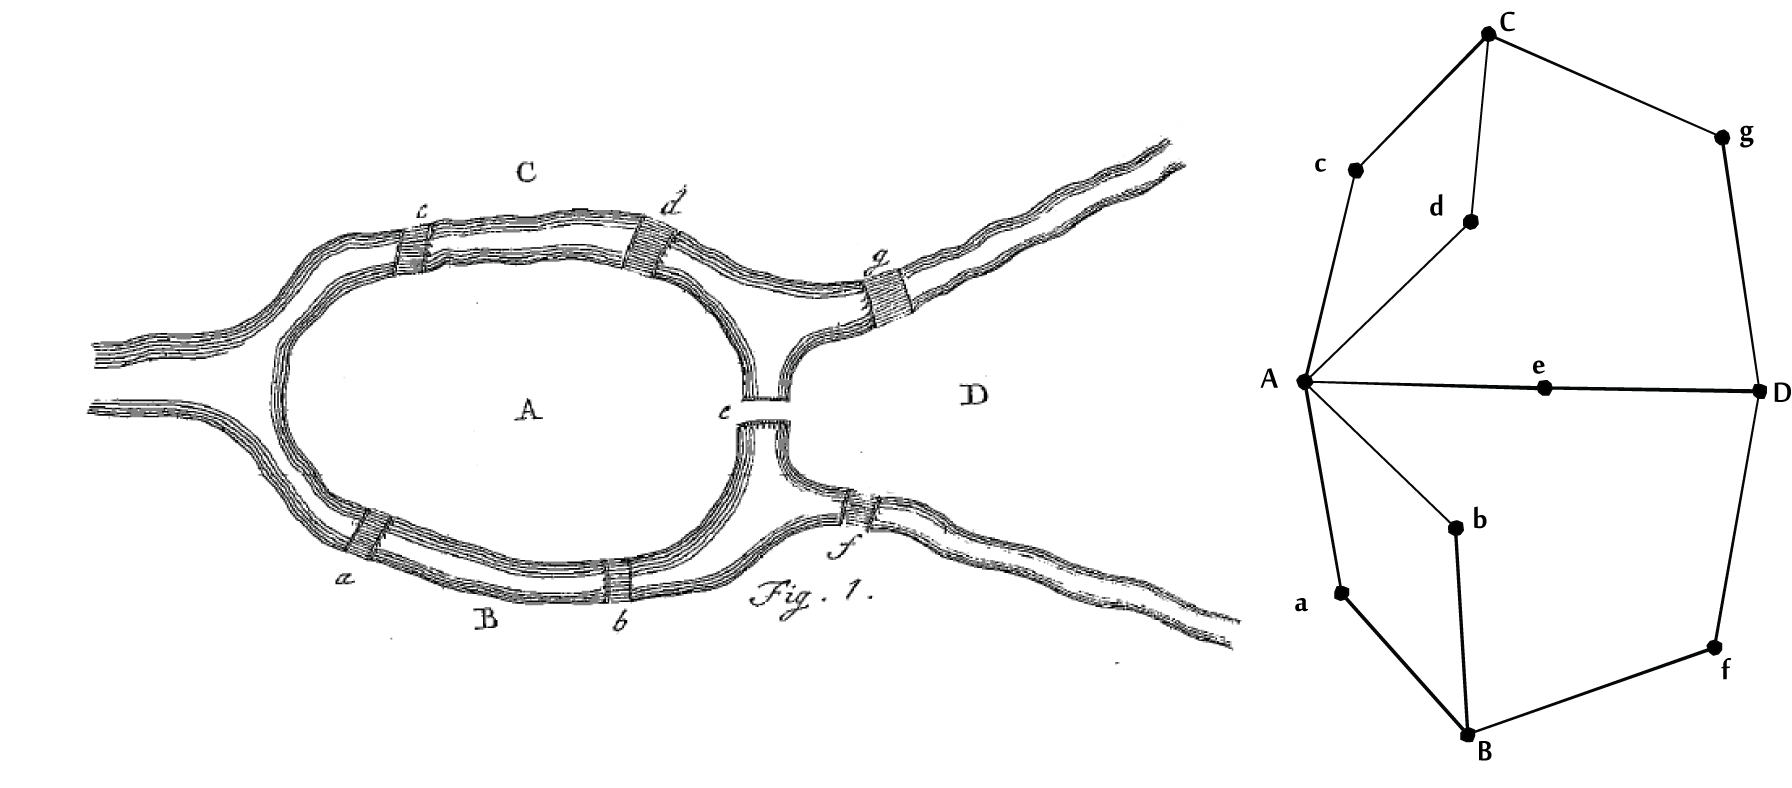
\includegraphics[width=0.9\textwidth]{./img/euler.png}
\label{fig:eulerbridges}
\end{figure}


The basic constructions of graph theory are straightforward.  A graph is a collection of objects called vertices \citep{Bollobaas1998} joined together with connections called edges.  The study of graphs is typically fruitful in any endeavor in which items may be either related or not, such as electronic circuit design \citep{Bollobaas1998},  protein interactions \citep{Palla2005}, social network analysis \citep{Knoke2008} and internet search \citep{Brin1998}.  

\section{Graph Theoretic Approach to Food Combinations}
A recent development in the search for optimal combinations of components takes a new approach, one based on relatively recent mathematical advances.  In particular, \citet{Ennisa} have proposed a graph theoretic approach to determining compatibility \citep[see also][]{Ennis2010, Ennis2011}.

To illustrate the use of graph theory in the study of food item compatibility, we view a list of 25 salad toppings as 25 vertices on a graph.  In this case, we consider vertices to be connected exactly when the salad toppings are compatible.  Our challenge of finding compatible larger collections of salad toppings can then be translated into the graph theoretic challenge of finding larger collections of vertices that are fully interconnected.  Such collections of vertices are called cliques.  In the case of subject response data, if the three pairwise combinations of ingredients Apple-Carrot, Banana-Carrot and Apple-Banana are compatible, then the larger combination or clique Apple-Banana-Carrot is a predicted compatible combination.  However, if one of the three pairs is not compatible, such as Apple-Carrot, then the larger combination is not a predicted combination (nor is it a clique).  

Using this clique finding technique, vast numbers of combinations can be eliminated from consideration, allowing the researcher to focus attention on a short of list of fully compatible combinations.  This method is not meant to supplant existing techniques but rather is meant to complement existing methods by helping researchers screen large numbers of combinations down to a reasonable size list that can then be analyzed in greater detail.  

\section{Research Program}
The goal of the current research program is to apply the \citet{Ennisa} graph theoretic approach to foods and to propose an extension to the approach for menus and to test the validity of a crucial assumption.  In particular, in any product category in which we wish to apply the graph theoretic approach, in order to justify the elimination of combinations that are not fully pairwise compatible and to reasonably focus only on combinations that are fully pairwise compatible (i.e. the cliques), we need to know that the following assumption holds:

\noindent
{\bf Principle of Supercombinatorality (SC):} Combinations that are fully pairwise compatible will be considered more compatible overall than combinations that are not fully pairwise compatible.

SC is so named as it asserts that compatible combinations can be super-constructed from compatible pairs.  In the language of food science, SC says that compatible food products can be constructed from compatible food components.  In the language of graph theory, SC says that cliques will be considered more compatible than non-cliques.
In doing so, we will validate the underlying psychological effect, the property of supercombinatorality, which allows us to take pairwise consumer response data and scale it up to larger combinations.  This novel approach is then extended to menu development where cross category comparisons are introduced and an analysis is proposed.  Finally, we show a method for ranking the results to provide more specific feedback to consumer scientists.  

\pagebreak
\renewcommand\bibname{{REFERENCES}} %  will print "REFERENCES" instead of "BIBLIOGRAPHY"
\phantomsection
\addcontentsline{toc}{section}{References} %  adds "REFERENCES" to the table of content
\bibliographystyle{apalike}
\bibliography{library_man}  % uses the references stored in Chapter1Radar.bib

\chapter{Study Objectives}
\section{Validating a Graph Theoretic Screening Approach to Food Item Combinations}

The aim of this study was to investigate and validate the concept that compatibility information on pairs of items, gathered via a consumer questioning procedure, can be used to predict larger combinations of items.  An important concept in this study was that this scaling up was tested at the individual level.  The validation of this scaling up at the individual level would give consumer researchers a new tool to investigate food combination consumption patterns.

\section{A Group Level Validation of the Supercombinatorality Property: Finding High-Quality Ingredient Combinations Using Pairwise Information}
The aim of this study was to extend the previous study by investigating the supercombinatorality property at the group level and with a new product system (pizza toppings).  This investigation showed techniques for combining individual pairwise response data into a group response matrix, which was then used to create predictions. These predictions were then checked by the same individuals.  If this study were successful it would show how to validate the supercombinatorality property with ones’ own product system, as well provide the first results of the type of supercombinatorality study that could be used in real-world scenarios.  
\section{A Graph Theoretic Approach to US Army Field Ration Menu Development}
Menus are unique types of combinations of foods because, unlike pizza and salad ingredients, the items to be combined come from separate categories.  This study extended the graph theoretic approach to menu development using the Meal-Ready-to-Eat\tm and also introduced a ranking system for proposed combinations to predict their potential success.  Being able to predict menus from pairwise responses would allow researchers to overcome complex problems related to other menu development approaches and provide a comprehensive toolkit for investigating combinations of foods.

\chapter{Validating a Graph Theoretic Screening Approach to Food Item Combinations}
\section{Abstract}
Tools from the mathematical field of graph theory potentially allow the consumer scientist to  efficiently analyze large numbers of combinations of food items, such as components on a salad.  In this study, we tested the validity of such an approach.  We began by asking subjects whether or not pairs of ingredients would be appropriate to combine on a salad.  Next, using graph theoretic methods, we predicted which combinations of 3-8 components should go together and, perhaps more importantly, which combinations should not.  Subjects were then asked whether or not particular combinations were appropriate to combine on a salad.  A paired Wilcoxon test between the predicted and non-predicted combinations was significant for all combination sizes.  

\section{Practical Applications}
A consumer driven graph theory methodology provides a screening tool to quickly and efficiently reduce a vast number of combinations of food items down to a reasonable number which can then be evaluated by the consumer scientist using suitability criteria together with more traditional tools.  In the case of salads, we screened over 1.7 million combinations and eliminated all but a handful as being unsuitable.  This methodology has potential in menu development, portfolio design and individual product formulations.  The advantage to the researcher is that the method can be inexpensively performed, is non-biased and is comprehensive.  This study validates the use of this approach in a particular screening application.

\section{Introduction}
The challenge of finding optimal combinations of food items, an important problem with effectively unlimited commercial applications, has been visited repeatedly with varying levels of success.  For instance, \citet{Eindhoven1959} observed that the prediction of peoples’ preferences for combinations of food items, such as menu items, was more complex than just a linear additivity of the preference for the individual items.  Factors such as texture, color and separation of items \citep{Eindhoven1959,Pilgrim1961}, context and consumer ethnicity \citep{Marshall2003,Niewind1986}, frequency of consumption \citep{Marshall2003} and hypo-additivity or the “a la carte” effect \citep{Lawless1994} have all been found to complicate this combinatorial effect.  In addition, there are considerable individual differences that lead to one’s hedonic feelings towards a particular food item.  Taste, over texture or appearance, is the strongest predictor of liking but this is by no means ubiquitous \citep{Moskowitz1995}.   Further, in \citet{Moskowitz1995}, overall liking was predicted poorly by liking of individual components (R\superscript{2} values of 0.4 - 0.7).  It follows that if immediate progress is to be made towards meeting this challenge, a simplification would be desirable, and it was in search of such a simplification that \citet{Worsley1984} had grade school students evaluate 780 pairwise combinations of food items and answer how well “the foods in each pair would go together to form a nice meal.”  

A classical approach to analyzing pairwise information is to employ multidimensional scaling (MDS); whether deterministic \citep{Schiffman1981} or probabilistic \citep{Ennis1988}; a method of creating visual perceptual maps from similarity data.  This MDS methodology has been extended with cluster analysis to find entr\'{e}es, starches and desserts that were close to each other, and followed by a regression analysis to predict compatibility ratings of the three component meal from the ratings given to the component pairs \citep{Klarman1977}.  A modified just-about-right scale \citep{Johnson1987} can also be used to evaluate optimal pairs of food items, and in the case of a wine and cheese pairing the two anchors would be “cheese dominates excessively” and “wine dominates excessively” with an “ideal match” point in the center \citep{King2005}.  \citet{Niewind1986} used a novel dual-scaling analysis \citep{Nishisato1984}, rather than MDS to analyze pairwise similarity categories on 39 different side dishes with 4 different main items.  Dual scaling (also known as Correspondence Analysis or CA) provides a way of quantifying and testing for significant differences between categorical data, such as complex questionnaires.

Regression analysis adds predictive capabilities to meal acceptability combination data.  The regression equations typically take on some variation of this form, where meal acceptability data of the individual components predicts whole meal results \citep{Hedderley1995,Moskowitz1983,Turner1988}:

\begin{equation}
Whole Meal = \beta _{0} + \beta _1(Appetizer) + \beta _2(Entree) + \beta _3(Dessert)\
\nonumber
\end{equation}
	
Modifications to the regression equation have been applied to the application of cyclic menus by means of a squared coefficient \citep{Moskowitz1983} for time since last presentation.  One of the effects noted above for combinations of food items is that scores are not additive.  

A more complex regression based method is conjoint analysis, which presents whole product concepts containing multiple elements or effects (packaging design, suggested time of eating, flavors, etc.) \citep{Green1978}.  Multiple concepts containing presence or absence of multiple values or levels of each of the different effects are presented to each subject and are either rated on a scale or as a binary accept/reject.  Regression analysis is used to determine the individual worth of each element towards the entire concept, and the model can then be used to find the best performing combination of attributes \citep{Moskowitz2006a}.  Conjoint analysis is strongly influenced by the axioms presented by \citet{Luce1964} which set a mathematical groundwork for what \citet{Luce1964} called conjoint measurement and justified the breaking down and recombining of individual effects to create an overall model.  One of the criticisms of conjoint analysis is that the concepts presented to the subjects must be derived by the practitioner and elements combined in such a way as to make them all independent of each other in the subsequent analysis.  A conjoint analysis measurement containing multiple effects and multiple levels, therefore, can have hundreds or thousands of different concepts to present to a consumer, which is a mentally challenging task and also greatly dependent on the abilities of the practitioner to design a good test.

In this paper, we explore an alternative approach to tackling problems involving pairs and combinations based on recent advances in mathematics and computer science, specifically in the field of graph theory \citep{Ennisa,Ennis2010,Ennis2011}.   We will see that graph theory emphasizes connections between items, rather than attributes of the items themselves and thus provides a novel perspective to explore this area of perception.  In particular, \citet{Ennis2010} have proposed a consumer driven methodology utilizing graph theory to approach our original challenge of finding optimal combinations of food items.  The choice of individual items is extremely flexible; items can be individual flavors, ingredients, pizza toppings, components of a ready to eat meal, etc.  This method is not meant to replace existing methodology but instead is meant to complement methods already in use by helping researchers screen a potentially astronomical number of combinations down to a manageable number that can then be studied using existing tools.  For example, if a consumer packaged goods company is developing a new frozen pizza, has 25 pizza toppings at their disposal and is interested in pizzas with  between two and eight toppings, there are 1,807,755 possible pizzas to consider.  Traditional strategies employed for screening these hypothetical pizzas for additional consideration typically include: discussion among a small committee of people, previous sales data, or in some cases consulting a single individual who is deemed to be an expert.  But these strategies, with the exception of conjoint approaches, are rarely consumer driven.

The technique we investigate is one of asking for pairwise information regarding item compatibility.  From this pairwise information, such as that collected by \citet{Worsley1984} and mentioned earlier, we use techniques from graph theory to build larger combinations suitable for additional examination using existing tools.  A vast number of unsuitable combinations will be eliminated from consideration allowing us to avoid the problem size issues experienced by conjoint based approaches.  As a metric for suitability, we will use appropriateness \citep{Schutz1988}, a concept that stems out of the development that acceptance is unpredictable and is not a great predictor of consumption \citep{Sidel1972}. By analyzing combinations under appropriateness conditions, the graph theory method explored in this paper maximizes external validity, rather than using hedonic ratings as a surrogate for whether or not people will consume an item.  The idea is to gather appropriateness information for pairs of items and then use mathematical tools to find combinations of items that are fully pairwise appropriate.  This technique will allow us to produce a short list of combinations worthy of additional investigation.  But the question remains, “Is this graph theoretic technique actually effective in practice?”  In other words, “Is it true that screened-out combinations are generally of low quality while combinations that survive the screening process are generally of high quality?”.  The contributions of this paper are then two-fold.  In particular we show in this paper that for a particular product category that the answers to the above questions are both “yes.”  But, more generally and more importantly, we demonstrate through our example a process one might follow to verify that the graph theoretic screening technique we review is appropriate for other product categories.  Once this tool has been verified for a category, the time and cost savings provided by the use of graph theoretic screening are potentially great.  To this end, we begin by reviewing concepts from graph theory that we need to conduct our screening.  We then describe an experiment conducted in the fresh salad category before we present analysis demonstrating that, in this case, the screening technique was effective according to the criteria listed above.  

\section{Graph Theory}

The basic constructions of graph theory are straightforward.  A graph is a collection of objects called vertices \citep{Bollobaas1998} joined together with connections called edges.  See Figure~\ref{fig:exgraph} for an example of a graph with 8 vertices and 12 edges.  

\begin{figure}[h!]
\caption[Example graph.]{Graph with eight vertices and twelve edges.}
\centering
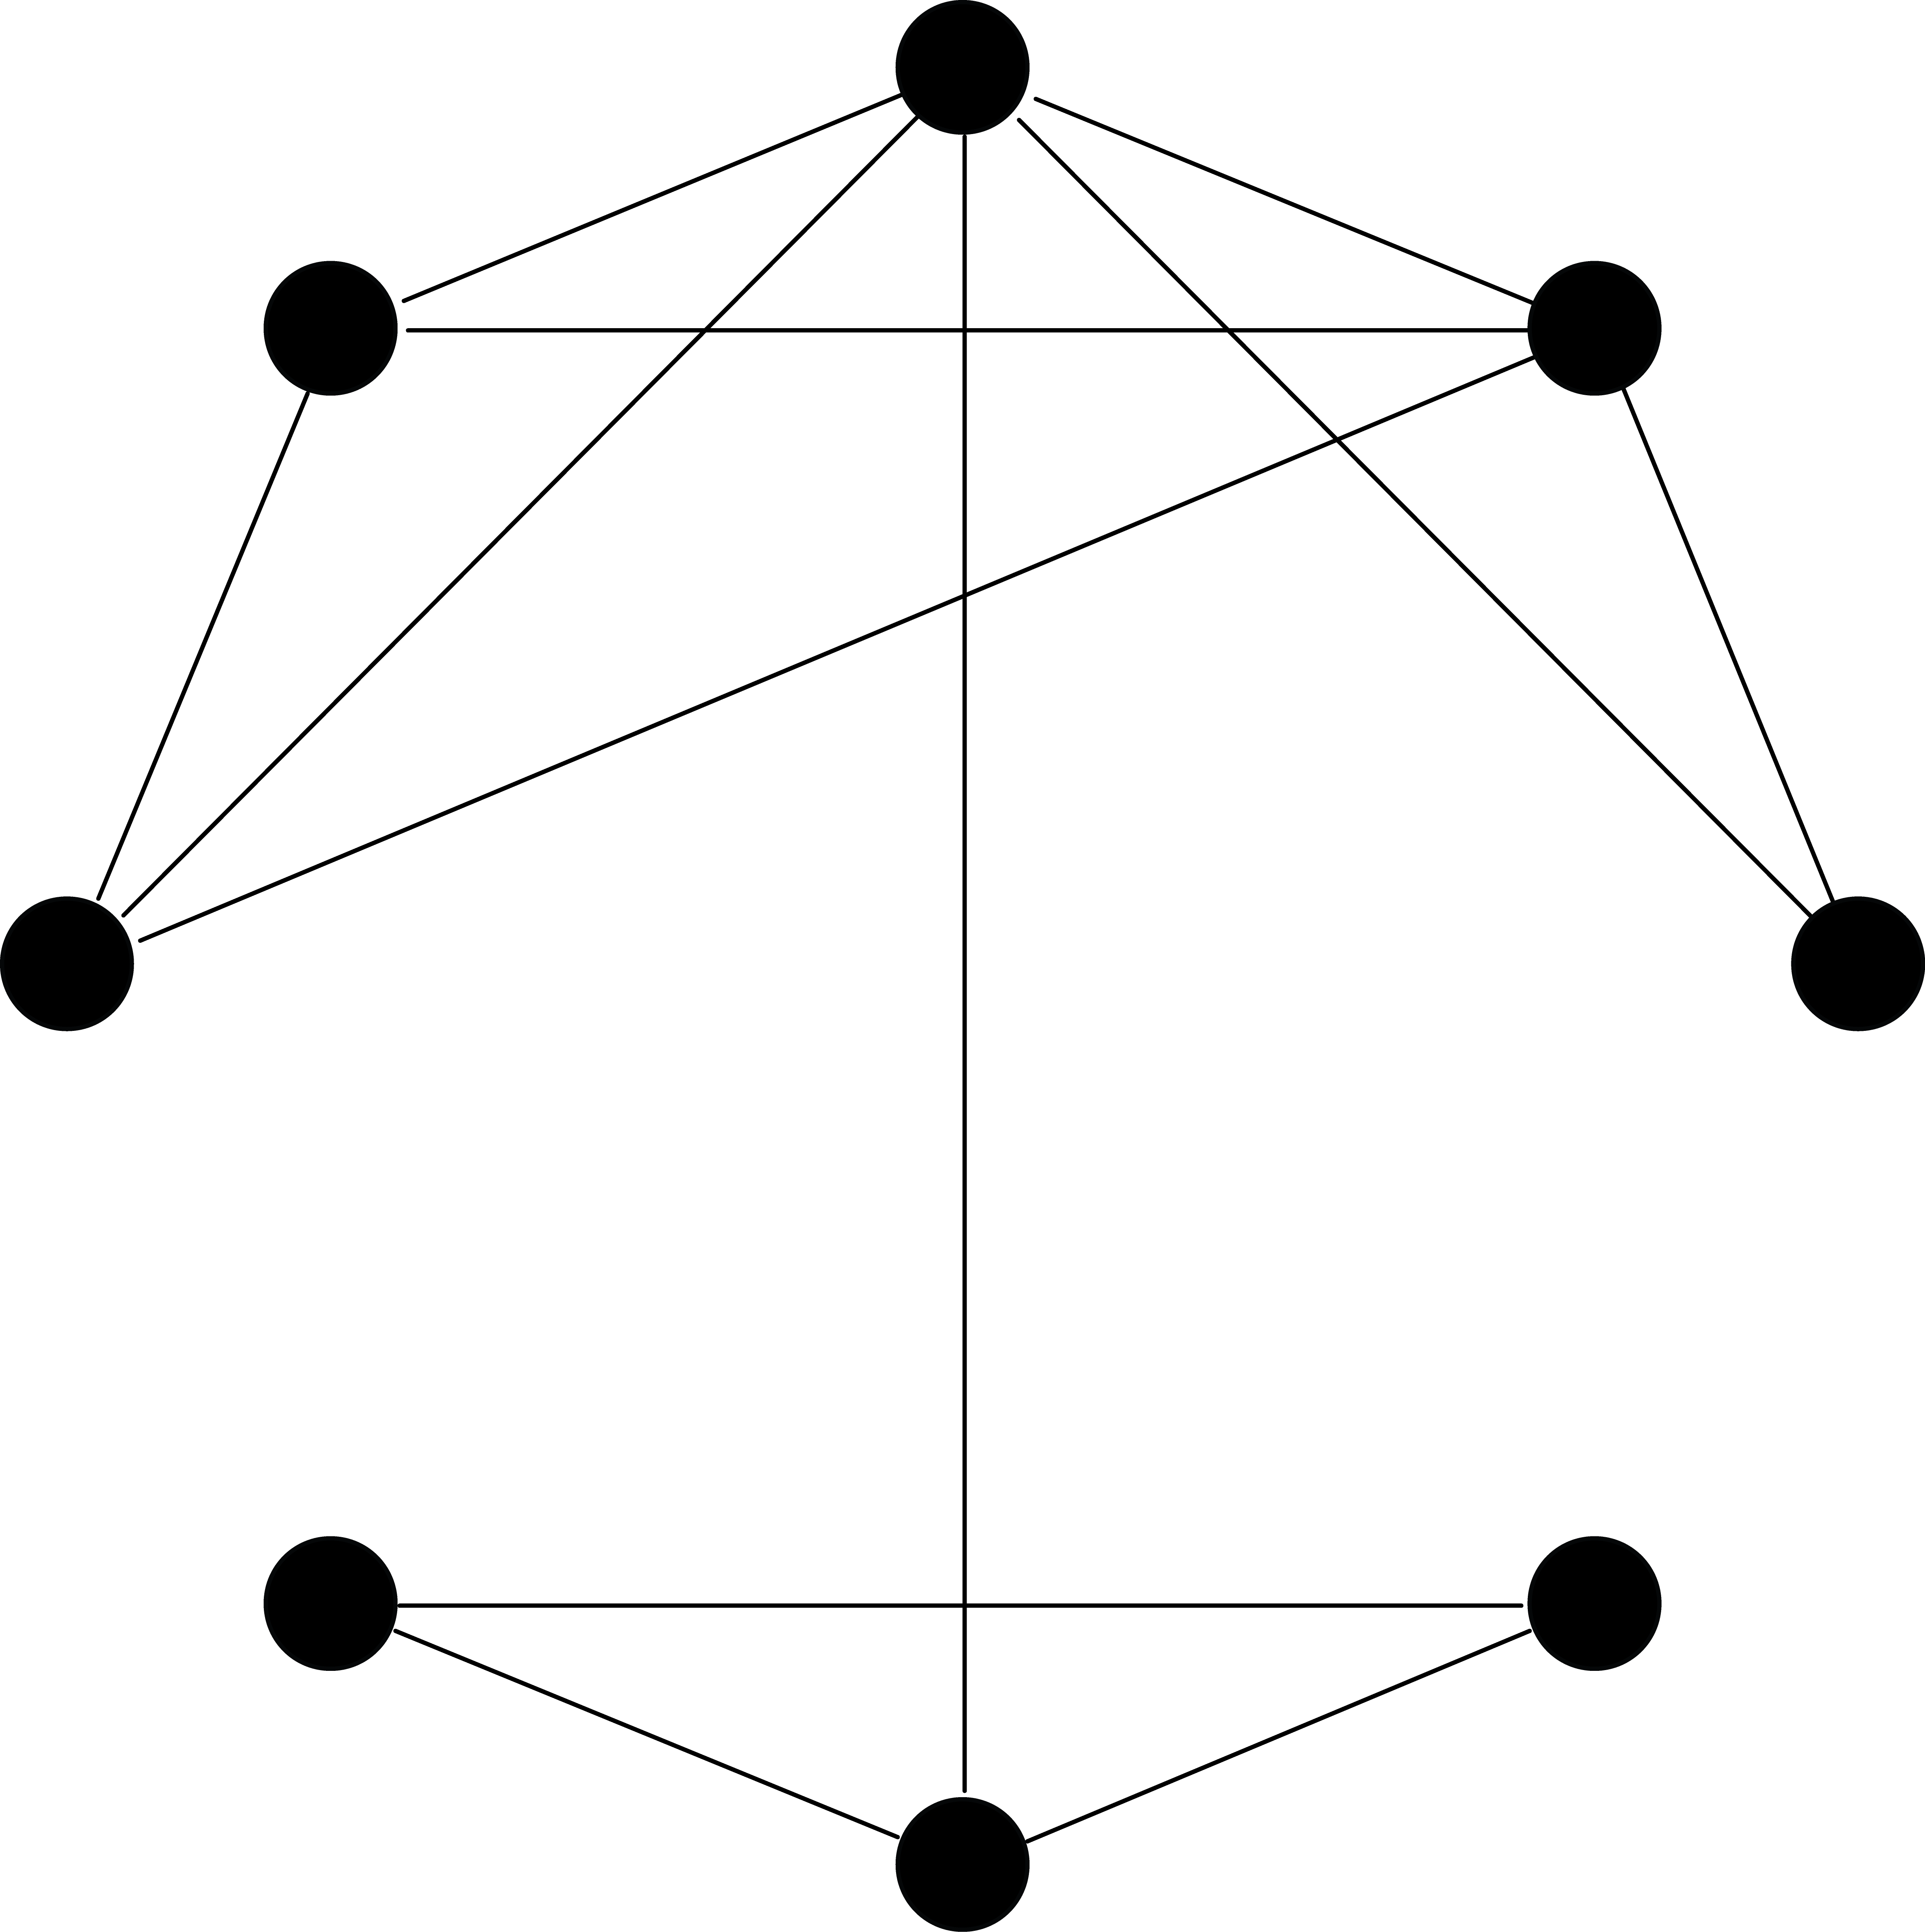
\includegraphics[width=.6\textwidth]{./img/basic_graph.png}
\label{fig:exgraph}
\end{figure}

The study of graphs is typically fruitful in any endeavor in which items may be either related or not, such as electronic circuit design \citep{Bollobaas1998},  protein interactions \citep{Palla2005}, social network analysis \citep{Knoke2008} and internet search \citep{Brin1998}.  To illustrate the use of graph theory in the study of food item compatibility, we view a list of 25 salad toppings as 25 vertices on a graph.  In this case, we consider vertices to be connected exactly when the salad toppings are compatible.  Our challenge of finding compatible larger collections of salad toppings can then be translated into the graph theoretic challenge of finding larger collections of vertices that are fully interconnected.  Such collections of vertices are called cliques.  In the case of subject response data, if the three pairwise combinations of ingredients Apple-Carrot, Banana-Carrot and Apple-Banana are compatible, then the larger combination or clique Apple-Banana-Carrot is a predicted compatible combination.  However, if one of the three pairs is not compatible, such as Apple-Carrot, then the larger combination is not a predicted combination (nor is it a clique).  Figure~\ref{fig:exmaxclique} shows the same graph as in Figure~\ref{fig:exgraph} with all of the (maximal) cliques highlighted.  For our salad example, we hypothesize: 1) cliques represent potential successful salads and 2) non-cliques represent unsuccessful salads that can safely be removed from future consideration.  An experimental validation of this hypothesis is the topic of our next section.  

\begin{figure}[h!]
\caption[Example graph with maximal cliques]{Graph from Figure~\ref{fig:exgraph} with maximal cliques circled.}
\centering
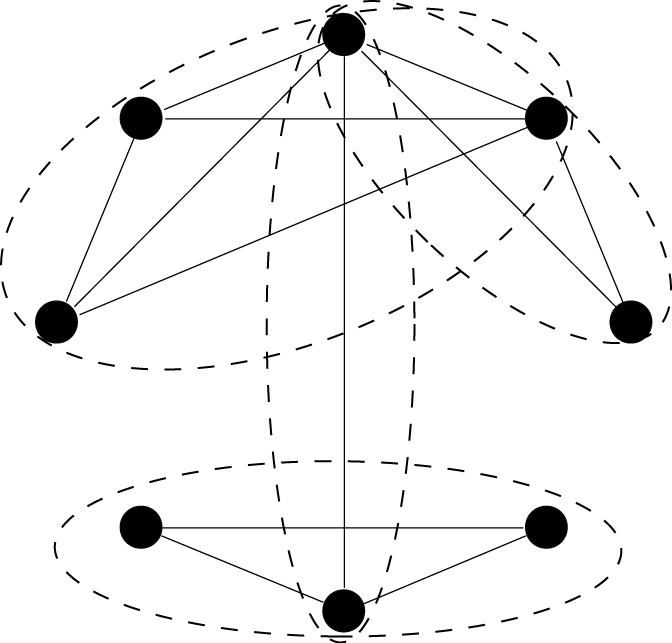
\includegraphics[width=0.6\textwidth]{./img/cliques.png}
\label{fig:exmaxclique}
\end{figure}

\section{Experimental Overview}
The study presented in this paper tests our hypothesis that combinations that are fully pairwise appropriate will be of high quality, i.e. will generally be judged as appropriate combinations, while those combinations that are not fully pairwise appropriate will be judged as inappropriate combinations.  In order to test this hypothesis, subjects were asked to provide appropriateness responses for pairwise combinations of 25 salad ingredients.  For each subject, their own complete set of cliques was formed.  Each subject was then asked whether or not it was appropriate to combine larger combinations of ingredients in a salad, using both cliques and random non-cliques for each size combination.  Our prediction was that the cliques method would perform significantly better than non-cliques.  

\section{Materials and Methods}
\subsection{Subjects}
105 responses were collected for an internet-based pre-survey (54 male), which gathered information on popular salad ingredients.  110 people participated in the main study.  Of those, 63 (22 male) were included in the final analysis.  The reason that 47 responses were excluded is because of the mathematical fact that if the subjects were too demanding or too accepting then there would not be enough cliques to test against the non-cliques, or conversely.  Thus, out of the 110 people whom completed the questionnaire, 63 continued on to the third part of the survey.  Prior to participation in the study, subjects were screened for regular salad consumption.  Subjects gave informed consent and this investigation was approved by the Cornell University Institutional Review Board.

\subsection{Pre-Survey Details}
The purpose of the pre-survey was to determine a list of 25 popular and familiar ingredients for use in the main survey.  An online questionnaire was developed which asked subjects to list the ingredients they would want in their favorite salad.  Panelists were recruited via department email lists and internet-based social networking websites. They were told that the salad included iceberg lettuce and no information was provided regarding a dressing.  Similar ingredients were combined (e.g. grilled chicken and chicken).  The final list is presented in Table~\ref{tab:salading}.


\begin{table}[h!b!p!]
\centering
\caption[25 popular salad ingredients]{25 popular salad ingredients determined from the pre-survey.  Similar ingredients were combined to produce a final list used in the subsequent supercombinatorial questionnaire.}
\begin{tabular}{cccc}
\toprule
\multicolumn{4}{c}{Ingredients} \\
\midrule
Tomatoes 		& 	Cucumbers 	& 	Carrots 	& 	Croutons 	\\
Bacon 			&	Blue Cheese 	& 	Spinach 	& 	Almonds 	\\
Chicken 		& 	Chickpeas 	& 	Feta Cheese 	& 	Onions 	\\
Sunflower Seeds 	& 	Black Olives 	& 	Broccoli 	&	Dried Cranberries \\
Hard-Boiled Egg 	& 	Cheddar 	& 	Mushroom 	& 	Avocado 	\\
Corn 			& 	Apples 		& 	Walnuts 	& 	Beets 		\\
Bell Peppers \\
\bottomrule
\label{tab:salading}
\end{tabular}
\end{table}

\subsection{Main Survey Details}
The survey for the second part of the study was conducted via computer at the sensory evaluation testing facility in the Cornell University Department of Food Science.  Custom software was developed by the Institute for Perception  to mimic a paper survey methodology with the addition of automated responses and analysis.  This allowed us to reduce panelist variability by performing the entire survey in a single session.  For Part 1, subjects were presented with the list of 25 ingredients, one at a time, and asked if under any circumstance they would consider consuming that ingredient on a salad.  If they chose no to any ingredient, that ingredient was removed from all subsequent parts of the survey for that subject.  

For Part 2, for each subject, all possible pairwise combinations from that subject’s remaining set of ingredients were generated.  For example, if a subjects selected 20 out of the 25 ingredients in Part 1, then 190 pairs were generated for Part 2.  The pairs were randomized in both overall order and with respect to presentation order within the pairs.  Subjects were asked, for each, to answer a YES/NO question as to whether or not they would consider the pair appropriate to combine together on a salad.  After appropriateness information regarding all pairs was collected, the software found cliques and non-cliques of sizes 3-8.  An equivalent number of cliques and non-cliques was presented for each, thus controlling for any size effect in the subsequent statistical analysis.  

For Part 3, the subjects were presented their own cliques and non-cliques (no more than 100 in each condition).  The order within and between sets of ingredients was again randomized.  In this part, as in Part 2, the subject was asked whether each combination was appropriate to combine on a salad and the software recorded the responses.  

\subsection{Data Analysis}
For the overall analysis we chose to combine maximal cliques and non-maximal cliques into a “clique” category.  When a combination was chosen by a subject to be appropriate, this was counted as compatible.  For each subject and for all subjects the total number of times a subject indicated that a combination was compatible for each of the two conditions - predicted compatible combinations (cliques) and predicted incompatible combinations (non-cliques)  - was counted.  The Wilcox paired rank sum test is a non-parametric test which can be used to evaluate whether or not two distributions of counts overlap or are separate.  This test was used to compare the two distributions being tested - predicted compatible vs. predicted incompatible - for all combination sizes.  All data analysis was performed in R 2.10.0 using the stats package.  

\section{Results}
\subsection{Pre-Survey}
The pre-survey successfully met our goals of determining a list of 25 popular salad ingredients, which are presented in Table~\ref{tab:salading}.  There were 161 unique ingredients ranging from obvious (mushrooms, cheddar cheese) to obscure (nacho flavored chips, sour cream).  The top 25 ingredients were agreed upon by at least 10 people at a minimum, with the tomatoes (\#1) being requested by 54 people.  

\subsection{Main Study}
To test our hypothesis that the graph theoretic screening is valid, we used pairwise compatibility ratings to predict larger combinations of food items by finding cliques.  Specifically, when cliques of 3+ food items were generated from pairwise compatibility ratings, we hypothesized that the proportion of people who would find the cliques appropriate would be significantly larger than the proportion of people who would find random non-cliques appropriate:  
\begin{align*}
 & H_o: P(clique) = P(non-clique)\\ 
 & H_a: P(clique) \neq P(non-clique)
\end{align*}

Figure~\ref{fig:saladgraph} shows a graph generated from the pairwise compatibility information from Panelist 1.  Each connection in the graph represents a “yes” response from the survey.  Immediately it is apparent that for this panelist some ingredients, such as bell peppers, are much more highly compatible than others, such as apples and avocado, represented by the number of edges in the graph connected to those nodes.  The clique finding algorithm found all fully interconnected combinations, or cliques, of 3 to 8 ingredients.  A subset of these maximal cliques, along with the tested non-maximal cliques and non-cliques is shown in Table~\ref{tab:ponesalad}.

\begin{figure}[h!]
\caption[A panelist's salad graph.]{Graph from a panelist showing pairwise connectivity information.  Apples and Bacon are less compatible than tomatoes and mushrooms.}
\centering

\includegraphics[width=0.9\textwidth]{./img/ind_super_pairgraph.png}
\label{fig:saladgraph}
\end{figure}

Table~\ref{tab:wilcoxsalad} shows the results from the overall Wilcoxon test used to assess predicted compatibility.  For every clique size, there is significant evidence in support of our hypothesis that the graph theoretic screening is valid.  It is particularly interesting to note that although one might expect less support for our hypothesis for larger combination sizes, given how far removed those combinations are from the pairwise information, we observe supporting evidence even for an eight component salad.   Out of the 63 subjects, only 3 chose more non-cliques than cliques as being compatible when summed over all combination sizes.  Proportions of people whom chose a greater number of cliques over non-cliques as being compatible are shown in Table~\ref{tab:propsalad}.

\begin{landscape}
\footnotesize
\begin{longtable}{lllllllll}
\caption[Panelist 1 Salad Combinations]{Salads for Panelist one with compatibility responses.} \\
\endfirsthead
\toprule
\endhead
\multicolumn{9}{c}{Continued on next page...} \\
\endfoot
\bottomrule
\endlastfoot
\bottomrule
\multicolumn{2}{l}{\bf Maximal Cliques} \\
\cmidrule(l){1-2}
Response & Item 1 & Item 2 & Item 3 & Item 4 & Item 5 & Item 6 & Item 7 & Item 8\\
\midrule
TRUE & Bell Pepper & Black Olive & Chicken & Cucumber & Blue Cheese & Broccoli  \\
TRUE & Chicken & Bacon & Mushroom & Bell Pepper \\
TRUE & Chicken & Bell Pepper & Mushroom & Tomato & Cucumber & Black Olive & Broccoli \\
\midrule
\multicolumn{2}{l}{\bf Non-Maximal Cliques} \\
\cmidrule{1-2}
Response & Item 1 & Item 2 & Item 3 & Item 4 & Item 5 & Item 6 & Item 7 & Item 8\\
\midrule
TRUE & Cucumber & Broccoli & Corn & Bell Pepper & Carrots & Tomato & Chicken & Mushroom \\
TRUE & Broccoli & Tomato & Onion & Corn & Chicken & Mushroom & Cucumber & Bell Pepper \\
TRUE & Corn & Cucumber & Chicken & Tomato & Bell Pepper & Carrot & Broccoli & Onion \\
TRUE & Chicken & Onion & Carrot & Cucumber & Mushroom & Tomato & Bell Pepper & Broccoli \\
TRUE & Tomato & Broccoli & Mushroom & Corn & Chicken & Cucumber & Onion & Carrots \\
TRUE & Bell Pepper & Chicken & Carrot & Mushroom & Cucumber & Onion & Broccoli & Corn \\
TRUE & Chicken & Tomato & Onion & Corn & Cucumber & Carrot & Mushroom & Bell Pepper \\
TRUE & Corn & Tomato & Bell Pepper & Broccoli & Carrot & Mushroom & Cucumber & Onion \\
TRUE & Carrot & Broccoli & Bell Pepper & Onion & Corn & Chicken & Mushroom & Tomato \\
\midrule
\multicolumn{9}{l}{\bf Non-Cliques} \\
\cmidrule{1-2}
Response & Item 1 & Item 2 & Item 3 & Item 4 & Item 5 & Item 6 & Item 7 & Item 8\\
\midrule
TRUE & Bell Pepper & Bacon & Avocado & Carrot & Cucumber & Blue Cheese & Onion & Black Olive \\
TRUE & Bell Pepper & Bacon & Avocado & Corn & Cucumber & Broccoli && \\
FALSE & Sun. Seeds & Blue Cheese & Bell Pepper & Carrot & Apple & Mushroom & Onion & Cucumber \\
FALSE & Cucumber & Onion & Corn & Black Olive &&&& \\
TRUE & Broccoli & Apple & Chicken & Tomato & Bacon & Carrot & Cucumber & \\
TRUE & Corn & Avocado & Onion & Carrot & Apple & Black Olive & Broccoli & Chicken \\
TRUE & Onion & Avocado & Black Olive & Corn & Blue Cheese & Tomato & Cucumber & Broccoli \\
TRUE & Corn & Broccoli & Chicken & Tomato & Blue Cheese & Bell Pepper & Tomato & Broccoli \\
FALSE & Tomato & Sun. Seeds & Corn & Mushroom & Onion & Apple & Chicken & Black Olive \\
TRUE & Onion & Mushroom & Black Olive & Cucumber & Blue Cheese & Bell Pepper & Tomato & Broccoli \\
FALSE & Blue Cheese & Bacon & Tomato & Carrot & Apple & Mushroom & Broccoli & Sun. Seeds \\
TRUE & Bacon & Bell Pepper & Cucumber & Sun. Seeds & Black Olive & Apple & Mushroom & Avocado
\label{tab:ponesalad}
\end{longtable}
\end{landscape}

\begin{table}[h!b!p!]
\caption[Wilcoxon Test Results]{Results summary from paired Wilcoxon signed rank test.  Counts of how many times subjects chose non-cliques were compatible were compared to counts of how many times subjects chose cliques to be compatible.  In all combination sizes tested, clique compatibilities were significantly higher than non-cliques compatibilities.}
\centering
\begin{tabular}{cccc}
\toprule
{\bf Combination Size} & {\bf P(clique)} & {\bf P(non-clique)} & {\bf Wilcox p-value} \\
\midrule
3 & 0.52 & 0.26 & 0.025 \\
4 & 0.54 & 0.28 & 0.023 \\
5 & 0.79 & 0.52 & 0.016 \\
6 & 0.90 & 0.46 & \textless 0.001 \\
7 & 0.79 & 0.55 & 0.006 \\
8 & 0.93 & 0.53 & \textless 0.001 \\
\bottomrule
\end{tabular}
\label{tab:wilcoxsalad}
\end{table}

\section{Discussion and Conclusion}
A graph theoretic approach to determining optimal food combinations is a novel approach that shows promise in addressing difficult problems in consumer research.  In particular, the graph theoretic technique for screening out inappropriate combinations described in this paper stands to augment existing techniques by allowing researchers to quickly and easily arrive at a small list of reasonable candidates that may then be examined using existing techniques.  In this paper we have presented results demonstrating the validity of a graph theoretic screening approach for the fresh salad category.  Showing that this approach is valid in other categories will be an important and necessary step in the investigation of these graph theoretic techniques.  The design presented in this paper, in which subjects were queried first regarding appropriateness of pairs of items and later regarding the appropriateness of larger combinations of items, both cliques and non-cliques, can be used to test the validity of graph theoretic screening in other product categories.  

As can be seen by Table~\ref{tab:propsalad}, some individuals do prefer non-cliques, and some predicted cliques were not compatible.   Thus it is possible that a good combination could be missed by this approach (Type II error), or a predicted combination could fail (Type I error).  However, this method does reduce the chance of both kinds of error.  Further manual screening of predictions is a recommended approach to help protect against Type I error.    

\begin{table}[h!b!p!]
\caption[Proportions of people whom preferred cliques over non-cliques to be compatible.]{Proportions of people who overall chose more cliques than non-cliques to be compatible for each tested combination size.}
\centering
\begin{tabular}{cc}
\toprule
{\bf Combination Size} & {\bf P(compatible)} \\
\midrule
3 & 0.82 \\
4 & 0.77  \\
5 & 0.77 \\
6 & 0.92 \\
7 & 0.75 \\
8 & 0.96  \\
\bottomrule
\end{tabular}
\label{tab:propsalad}
\end{table}

There are a number of potential improvements to the method.  Our compatibility response data are binomial (Yes/No).  Scaling of response data does offer an alternative which may increase sensitivity and reduce the number of subjects needed for stabilized results.  Another potential improvement would be to allow subjects to taste individual items during the test as desired to familiarize or re-familiarize themselves with the components, as this investigation operated under the assumption that everyone tested whom was a salad consumer was familiar with all of the items.

As a final point, it is worth noting that in our present study, we focused on whether or not graph theoretic screening is valid at an individual level since the cliques we presented subjects were based on their individual compatibility responses for pairs of items.  Testing whether or not graph theoretic screening is valid at a group level is an additional important step in this research program.  Such group level testing will be the topic of future research.    

\pagebreak
\renewcommand\bibname{{REFERENCES}} %  will print "REFERENCES" instead of "BIBLIOGRAPHY"
\phantomsection
\addcontentsline{toc}{section}{References} %  adds "REFERENCES" to the table of content
\bibliographystyle{apalike}
\bibliography{library_man}  % uses the references stored in Chapter1Radar.bib
\chapter{A Group Level Validation of the Supercombinatorality Property: Finding High-Quality Ingredient Combinations Using Pairwise Information}

\section{Abstract}

This study tested the principle of supercombinatorality,  i.e. that food combinations (of more than two items) that are fully compatible on a pairwise basis are more compatible than combinations that are not fully compatible pairwise.  Previous work has shown this to hold for salad ingredient combinations predicted for individuals, but this has not yet been tested for groups.  This study extended the previous findings to group data, and in a different product system, namely pizza toppings.  Purchase intent responses to pairs of 25 different pizza toppings were collected and used to predict pizzas (with one to 6 toppings) that would appeal to the entire group.  Results showed purchase interest to be higher for the predicted pizzas than for non-predicted pizzas supporting the supercombinatorality principle.  The study demonstrates that food product developers can use consumer-driven data and a graph theoretic approach to screen large numbers of potential food combinations in order to predict successful combinations and to do so in a highly cost-efficient manner.

\section{Introduction}

All food products can be viewed as a item combinations, whether these items are flavors (e.g. orange and vanilla),  ingredients (e.g. caramel, sea salt, sucralose and Aceulfame K), components within a meal (e.g. entrée, starch and vegetable) or components within a menu item (e.g. inclusions in a salad or ice cream, or toppings on a pizza).  Analytical approaches to optimize combinations based on preference have been elusive \citep{Eindhoven1959}, in part due to the vast numbers of possible combinations.  For example, if one is trying to find an optimally liked pizza containing between one and six toppings, and there are twenty-five unique toppings to choose from, there are almost one quarter of a million possible pizzas to consider.  It is not within the realm of traditional consumer testing methods to explore this problem exhaustively and as a result the most common method for solving the problem above is to use a consensus of a few product developer, research chefs or marketing analysts to decide what would be optimal combinations.  To remedy this situation, we seek a method with the following properties: 1) It must be complete: Every possible combination should be given the opportunity to be evaluated.  2) It must be consumer driven: There are obvious problems to using a panel of “company experts” to decide what consumers want.  3) It must be consumer friendly: The consumer must be able to perform the evaluation in a reasonable amount of time and with reasonable effort.  

Previous approaches to this type of problem primarily used regression based analyses \citep{Hedderley1995,Moskowitz1983,Turner1988}.  In the basic model, acceptability of the entire combination is predicted by acceptability of the individual components comprising the combination, such as entrée, starch and vegetable.  However, less than optimal results have been achieved \citep{Eindhoven1959}.  Overall preference is influenced by factors introduced by the combination itself, such as texture contrasts and color \citep{Eindhoven1959,Pilgrim1961}, context \citep{Marshall2003,Niewind1986}, and an “a la carte” effect \citep{Lawless1994}.  For example, the a la carte effect is a cognitive economic effect where people tend to discount the overall scores of groups of items over the sum of the scores of the individual items.  This was shown to exist in the context of how many of the Desert Bar snack products that soldiers would trade for either individual food stuffs from army field rations or for the entire ration, and from this it is suggested that this effect can and does contribute to the error associated with these regression analyses.  This basic regression approach could lead to the following hypothetical scenario where students rate overall liking on components for a meal.  Individually, spaghetti, coleslaw and pretzels might all be highly liked, but there is not any good justification for combining these together to create a meal, even though a regression model might predict it.  

Conjoint analysis is a more popular extension of the regression approach which has achieved a level of success in the consumer sciences \citep{Green1978,Moskowitz2006}.  In conjoint analysis, subjects are presented with scenarios comprising of multiple factor levels of variables (e.g. color and sweetness).  In a traditional conjoint model, a paired comparison questioning procedure presents two scenarios and subjects choose which scenario they like better.  Modifications have been developed which allow for scaling rather than 9-point hedonic scales \citep{Jones1955} to compare scenarios.  Most recently, experimental choice menus allow for subjects to select from a “choiceboard” particular components or features that appeal to them, which more closely models how we might select courses from a restaurant menu \citep{Liechty2001}.  For all models, regression approaches calculate the importance of each factor level to the overall concept.  Optimal concepts can then be predicted based on the results.  An important design consideration of the conjoint approaches is in the scenarios: factor levels must be chosen systematically in order to ensure balanced results.

A recent development in the search for optimal combinations of components takes a new approach, one based on relatively recent mathematical advances.  In particular, \citet{Ennisa} have proposed a combinatorial approach to determining compatibility \citep[see also][]{Ennis2010,Ennis2011} that uses tools from the mathematical field of graph theory \citep{Cazals2005,Valiente2002}.  According to this procedure, subjects answer binary (YES/NO) compatibility questions for all possible pairs of components being investigated.  For example, if an investigation seeks best combinations of yogurt flavors, with ten flavors under investigation there are forty-five pairs of flavors that can be formed out of the ten possible flavors.  Each subject then answers forty-five questions regarding the compatibility of each pair.   This small amount of data is then used to garner information regarding the 1024 possible combinations of flavors using the following approach:

\noindent
1) Each pair is classified as “compatible” or “incompatible” according to the proportion of respondents that considered the pair compatible.  The threshold level for proportions, above which pairs are considered “compatible,” depends on the goals of the study and is instance-specific.

\noindent
2) Cliques (combinations that are fully pairwise compatible) are found using graph theoretic techniques (Moon and Moser, 1965), and combinations that contain even one pair of items that are considered pairwise incompatible are eliminated from consideration. 

Following graph theoretic convention \citep{Moon1965}, combinations that are fully pairwise compatible are called cliques.  For example, suppose we have three flavors: Apple, Banana and Carrot.  If the flavor pairs Apple-Banana, Banana-Carrot and Apple-Carrot are all considered compatible then the combination Apple-Banana-Carrot is fully pairwise compatible and hence is called a clique.  On the other hand, if one of the pairs, Apple-Banana, was not considered compatible then Apple-Banana-Carrot would not be fully pairwise compatible and would not be considered a clique.  Note that clique finding for small numbers of flavors, or items more generally, can perhaps be conducted by hand, but for large numbers of items advanced algorithms are required.  For instance, if there are 20 flavors there are more than a million possible flavor combinations.

Using this clique finding technique, vast numbers of combinations can be eliminated from consideration, allowing the researcher to focus attention on a short of list of fully compatible combinations.  This method is not meant to supplant existing techniques but rather, in a manner similar to response surface \citep{Mullen1979} and fractional factorial \citep{Mullen1985} designs, is meant to complement existing methods by helping researchers screen large numbers of combinations down to a reasonable size list that can then be analyzed in greater detail.  An advantage of the graph theoretic approach over response surface or fractional factorial designs is that all item combinations are represented equally to the respondents, albeit indirectly.  

The clique finding or graph theoretic approach, while promising, depends on a crucial assumption.  In particular, in any product category in which we wish to apply the above approach, in order to justify the elimination of combinations that are not fully pairwise compatible and to reasonably focus only on combinations that are fully pairwise compatible (i.e. the cliques), we need to know that the following assumption holds:

\noindent
{\bf Principle of Supercombinatorality (SC):} Combinations that are fully pairwise compatible will be considered more compatible overall than combinations that are not fully pairwise compatible.

SC is so named as it asserts that compatible combinations can be super-constructed from compatible pairs.  In the language of food science, SC says that compatible food products can be constructed from compatible food components.  In the language of graph theory, SC says that cliques will be considered more compatible than non-cliques.

The first use of the graph theoretic approach for investigating food items \citep{Nestrud2010a} tested whether or not SC holds at the level of individual subjects.  In that study, subjects completed a pairwise questionnaire assessing the compatibility of twenty-five salad ingredients.  Clique-based salads of three to eight ingredients were found based on the individual subject’s responses and subjects were asked to assess both these clique-based salads as well as salads based on random non-cliques. The performance difference between the cliques and non-cliques was significant for all combination sizes.  For example, for the size eight combinations, i.e. the salads with eight toppings, the difference in proportions of subjects choosing the cliques vs. non cliques as compatible was 40\%, with the cliques reported compatible over 90\% of the time.  Thus the SC effect was validated in this instance at the individual level.  However, products are typically developed for groups rather than to satisfy individual particular consumers.  Therefore it is important to validate supercominatorality at the group level, which we demonstrate in this paper for the pizza category.  The study also provides an outline that can be followed for other product categories.  Validation in other categories would allow the product developer to be confident that potentially viable combinations are not ignored and also to find surprising combinations with innovative promise.

\subsection{Experimental Overview}
The study we describe in this paper tests our hypothesis that SC holds at a group level.  In particular, we developed a procedure for gathering pairwise compatibility information and for combining the responses from all of our subjects together.  We used a hypothetical scenario to predict a selection of highly liked pizzas based on cliques and validated our prediction by comparing these predicted pizzas to non-predicted pizzas based on non-cliques.  First, an internet survey gathered information on which pizza toppings were popular.  The top twenty-five toppings from this survey were used for the subsequent investigation.  Subjects answered pairwise compatibility questions based on a survey containing all possible pairs of the  twenty-five toppings.  Using the combined group responses, we predicted larger combinations, or cliques, of size three through six of toppings that were expected to be compatible according to SC.  To add resolution to our subsequent analysis, we divided these predicted combinations into two groups, maximal cliques and the non-maximal cliques.  A maximal clique is one that is not contained in any larger clique.  A non-maximal clique, therefore, is necessarily contained within some larger clique..  We tested each of these groups separately to distinguish if there were any unique properties of maximal cliques or non-maximal cliques related to the SC effect.  A third group, one of non-cliques, was created as a control group.  A non-clique was a combination of pizza toppings where at least one pair from the combination was not considered compatible.  

\section{Materials and Methods}
\subsection{Subjects}
100 subjects (29  male) completed the online survey.  The subjects were screened for both pizza consumption (at least monthly) and for whether or not they regularly consumed meat.  The reason the subjects were screened for meat consumption is that we did not want vegetarianism or perceived vegetarianism to be confounding factors.  For the main study, 124 subjects (48 male) completed Part 1 and 119 returned for Part 2.  These subjects were also screened for pizza consumption and whether or not they regularly consumed meat. The testing protocol was approved by the Cornell University Institutional Review Board and subjects gave informed consent.  

\subsection{Internet Pre-Survey}
Panelists were recruited from online social networking websites as well as from internal email recruitment lists.  The purpose of the survey was to develop a list of twenty-five popular pizza toppings.  For the reasons described above, we had subjects check off which meats they had consumed in the past year from a comprehensive list of protein sources (e.g. beef, pork, lamb, fish, etc.).  Subjects whom did not consume any meats were not used in the subsequent analysis.  It is also worth noting that  there is a recent trend of gourmet pizzas with non-traditional sauces, such as parmesan cream or pesto.  To avoid this potential confounding factor, the subjects were told that for the purposes of the survey the pizza was a traditional tomato sauce based pizza with mozzarella cheese.  The subjects were then asked to list what toppings they would choose on the pizza if cost was not an issue.  The top 25 ingredients by frequency of appearance were calculated (Table~\ref{tab:pizzaing}).

\begin{table}[h!b!p!]
\caption[Top 25 pizza ingredients from survey.]{Ingredients were determined in a survey of popular pizzas.  Similar ingredients, such as “garlic” and “roasted garlic” were combined.}
\centering
\begin{tabular}{cccc}
\toprule
\multicolumn{4}{c}{Ingredients}\\
\midrule
Anchovy 	& 	Artichoke 	& 	Bacon 		& 	Basil \\
Black Olive	& 	Broccoli 	& 	Chicken 	& 	Eggplant \\
Feta 		& 	Green Bell Pepper &	Ground Sausage & 	Ham \\
Italian Sausage & 	Jalapeno 	& 	Mushroom	&	Onion \\
Pepperoni 	& 	Pineapple 	& 	Prosciutto 	& Red Bell Pepper \\
Red Onion 	& 	Ricotta Cheese & 	Roasted Garlic & Spinach \\
Tomato \\
\bottomrule
\end{tabular}
\label{tab:pizzaing}
\end{table}

\subsection {Survey Details - Part 1}
All three hundred possible pairs of the twenty-five ingredients in Table~\ref{tab:pizzaing} were generated.  Paper based surveys then asked the subjects to check YES or NO as to whether or not they perceived the two ingredients to be compatible on a traditional pizza.  Using purchase intent as a proxy for compatibility, the specific question was: 

\noindent
{\it For each row on the following pages, please indicate whether you would or would not purchase a pizza if the one they have for sale has the toppings listed. Please do not purchase the pizza if you do not intend to consume all of the toppings (e.g. please do not plan on picking off a topping you do not like).}

Both the order of the pairs and the order of the ingredients within the pairs were randomized for each person.  Subjects were recruited to come to the sensory testing facility at Cornell University where they completed Part 1.

\subsection{Survey Details - Part 2}
Responses from Part 1 were combined together by counting the total number of times a pair was determined to be compatible.  These counts were input in a triangular similarity matrix of all twenty-five ingredients (Table~\ref{tab:pizztri}).  This matrix was then used to generate cliques as follows.  First, for a series of hypothesized thresholding values,  counts equal to or above threshold were taken to indicate compatibility between pairs while counts below threshold were taken to indicate incompatibility.  For each threshold value, the maximal cliques were determined using graph theoretic techniques.  Since our pre-survey indicated that pizzas with more than six toppings were undesirable, we chose as our final threshold the smallest threshold that gave cliques of size six but none of size seven.  As the threshold is decreased, more pairs are considered compatible and hence more and larger cliques will be formed.  In particular, our choice of threshold was 78 out of 124.  From this analysis, a list was generated of all of the maximal cliques  ranging in size from one to six.  The complete set of maximal cliques is presented in Table~\ref{tab:pizzmax}, and note that from this list all cliques and non-cliques can be determined.  




\begin{landscape}
\footnotesize
\begin{longtable}{cccccccccccccccccccccccc}
\caption{Triangular matrix of pizza ingredient compatibilities.} \\
\label{tab:pizztri} \\
\toprule
&\begin{sideways}Anchovy\end{sideways} &\begin{sideways}Artichoke\end{sideways} &\begin{sideways}Bacon\end{sideways} &\begin{sideways}Basil\end{sideways} &\begin{sideways}Black Olive\end{sideways} &\begin{sideways}Broccoli\end{sideways} &\begin{sideways}Chicken\end{sideways} &\begin{sideways}Eggplant\end{sideways} &\begin{sideways}Feta\end{sideways} &\begin{sideways}Green Bell \end{sideways} &\begin{sideways}Sausage\end{sideways} &\begin{sideways}Ham\end{sideways} &\begin{sideways}Italian Sausage\end{sideways} &\begin{sideways}Jalapeno\end{sideways} &\begin{sideways}Mushroom\end{sideways} &\begin{sideways}Onion\end{sideways} &\begin{sideways}Pepperoni\end{sideways} &\begin{sideways}Pineapple\end{sideways} &\begin{sideways}Prosciutto \end{sideways} &\begin{sideways}Red Bell \end{sideways} &\begin{sideways}Red Onion\end{sideways} &\begin{sideways}Ricotta \end{sideways} &\begin{sideways}Roasted Garlic\end{sideways} \\
\endfirsthead
\midrule
&\begin{sideways}Anchovy\end{sideways}&\begin{sideways}Artichoke\end{sideways}&\begin{sideways}Bacon\end{sideways}&\begin{sideways}Basil\end{sideways}&\begin{sideways}Black Olive\end{sideways} &\begin{sideways}Broccoli\end{sideways} &\begin{sideways}Chicken\end{sideways} &\begin{sideways}Eggplant\end{sideways} &\begin{sideways}Feta\end{sideways} &\begin{sideways}Green Bell \end{sideways} &\begin{sideways}Sausage\end{sideways} &\begin{sideways}Ham\end{sideways} &\begin{sideways}Italian Sausage\end{sideways} &\begin{sideways}Jalapeno\end{sideways} &\begin{sideways}Mushroom\end{sideways} &\begin{sideways}Onion\end{sideways} &\begin{sideways}Pepperoni\end{sideways} &\begin{sideways}Pineapple\end{sideways} &\begin{sideways}Prosciutto \end{sideways} &\begin{sideways}Red Bell \end{sideways} &\begin{sideways}Red Onion\end{sideways} &\begin{sideways}Ricotta \end{sideways} &\begin{sideways}Roasted Garlic\end{sideways} \\
\endhead
\midrule
 \multicolumn{7}{c}{Continued on next page...} \\
\endfoot
\bottomrule
\endlastfoot
Artichoke&20&&&&&&&&&&&&&&&&&&&&&& \\
Bacon&17&56&&&&&&&&&&&&&&&&&&&&& \\
Basil&22&58&68&&&&&&&&&&&&&&&&&&&& \\
Black Olive&21&48&50&52&&&&&&&&&&&&&&&&&&& \\
Broccoli&18&52&63&65&54&&&&&&&&&&&&&&&&&& \\
Chicken&17&60&76&86&49&80&&&&&&&&&&&&&&&&&\\
Eggplant&17&50&46&61&46&61&59&&&&&&&&&&&&&&&& \\
Feta&16&58&69&80&58&70&76&63&&&&&&&&&&&&&&& \\
Green Bell Pepper&14&50&56&65&46&66&68&52&61&&&&&&&&&&&&&& \\
Ground Sausage&21&56&77&78&54&66&70&59&75&75&&&&&&&&&&&&& \\
Ham&18&51&78&74&57&70&67&51&69&68&78&&&&&&&&&&&& \\
Italian Sausage&18&59&78&83&54&63&74&59&77&77&82&79&&&&&&&&&&& \\
Jalapeno&14&27&35&35&31&30&39&30&30&35&38&39&42&&&&&&&&&& \\
Mushroom&25&64&76&79&63&78&82&61&71&69&82&85&81&38&&&&&&&&& \\
Onion&22&56&77&65&51&64&75&61&62&72&78&73&85&34&84&&&&&&&& \\
Pepperoni&17&45&81&80&57&65&71&53&69&73&81&79&89&36&88&76&&&&&&& \\
Pineapple&11&38&66&47&36&47&64&32&54&50&64&79&57&29&53&46&53&&&&&& \\
Prosciutto Ham&16&47&69&69&52&57&63&47&72&61&69&66&72&39&75&64&67&66&&&&& \\
Red Bell Pepper&23&53&72&73&55&67&76&61&67&71&77&73&79&40&77&79&74&49&63&&&& \\
Red Onion&20&54&73&60&53&61&65&57&64&66&77&70&79&33&76&49&72&42&61&72&&& \\
Ricotta Cheese&18&59&69&76&50&71&76&60&63&63&81&80&83&32&71&71&82&55&73&70&66&& \\
Roasted Garlic&22&58&76&85&59&80&86&68&76&71&87&80&90&33&87&82&87&50&75&84&73&78& \\
Spinach&22&58&72&75&57&66&77&60&77&66&77&69&74&29&77&75&64&45&61&76&63&79&78 \\

\end{longtable}
\end{landscape}


\begin{landscape}
\footnotesize
\begin{longtable}{rcccccc}
\caption[Complete set of maximal cliques used in Part 2.]{Complete set of maximal cliques used in Part 2. Rows are predicted pizzas that were tested for compatibility. Predictions were based on pairwise responses from the threshold-adjusted Part 1 survey data.} \\
\label{tab:pizzmax} \\
\toprule
Clique & \multicolumn{6}{c}{\bf Ingredients in maximal cliques} \\
\midrule
\endfirsthead
\toprule
Clique & \multicolumn{6}{c}{\bf Ingredients in maximal cliques} \\
\midrule
\endhead
\midrule
 \multicolumn{7}{c}{Continued on next page...} \\
\endfoot
\bottomrule
\endlastfoot
1 & Anchovy & & & & & \\
2 & Artichoke & & & & & \\
3 & Black Olive & &&&& \\
4 & Eggplant & & & & & \\
5 & Jalapeno & & & & & \\
6 & Prosciutto Ham & & & & &\\
7 & Bacon &  Pepperoni & & & &\\
8 & Basil & Feta Cheese &&&&\\
9 & Ham & Pineapple &&&&\\
10 & Green Bell Pepper & Tomato &&&&\\
11 & Italian Sausage & Red Onion &&&&\\
12 & Broccoli & Chicken & Roasted Garlic &&&\\
13 & Ricotta Cheese & Spinach & Tomato &&&\\
14 & Ham & Italian Sausage & Pepperoni & Ricotta Cheese &&\\
15 & Ham & Italian Sausage & Mushroom & Pepperoni & Roasted Garlic &\\
16 & Basil & Chicken & Mushroom & Roasted Garlic &tomato &\\
17 & Ground Sausage & Italian Sausage & Pepperoni & Ricotta Cheese & Tomato &\\
18 & Italian Sausage & Mushroom & Onion & Roasted Garlic & Tomato &\\
19 & Italian Suage & Onion & Red Bell Pepper & Roasted Garlic & Tomato &\\
20 & Basil & Italian Sausage &  Mushroom & Pepperoni & Roasted Garlic & Tomato \\
21 & Ground Sausage & Italian Sausage & Mushroom & Pepperoni & Roasted Garlic & Tomato \\
\end{longtable}
\end{landscape}

The survey for Part 2 resembled that of Part 1, including the instructions, with the exception that instead of presenting pairs we presented combinations of toppings.   Each person was presented with the complete set of maximal cliques presented in Table~\ref{tab:pizzmax}.  For every maximal clique of a given size, a matched size non-maximal clique and non-clique were also input into the survey. Because there were many possible non-maximal cliques and non-cliques, these were drawn randomly for each person from the corresponding population of non-maximal cliques and non-cliques.  As in Part 1, each survey was randomized both in the order of the combinations presented and the topping order within the combinations.  Each subject was presented with twenty-one maximal cliques, nineteen non-maximal cliques and fifteen non-cliques.  There were not an equivalent number of maximal cliques, non-maximal cliques and non-cliques in each survey due to the mathematical nature of cliques.  All cliques of size six were maximal, therefore there were only non-cliques and maximal cliques of size six, but no non-maximal cliques.  Similarly,  there were no non-cliques of size one, as by definition unique ingredients form cliques.  The distribution of combination sizes for each person is listed in Table~\ref{tab:pizzdesign}.

\begin{table}[h!b!p!]
\caption[Size and distribution of combinations used in second survey.]{Size and distribution of combinations used in second survey. Values represent counts of purchase intent questions that were asked for combinations of a given size.  The maximal cliques were constant for everyone. Non-maximal cliques and non-cliques were chosen 
randomly for each person from all possible combinations within the category.}
\label{tab:pizzdesign}
\centering
\begin{tabular}{cccc}
\toprule
{\bf Combination Size} & {\bf Max Cliques} & {\bf Non-max Cliques} & {\bf Non-Cliques}  \\
\midrule
1 & 6 & 6 & 0 \\
2 & 5 & 5 & 5 \\
3 & 2 & 2 & 2 \\
4 & 1 & 1 & 1 \\
5 & 5 & 5 & 5 \\
6 & 2 & 0 & 2 \\
\bottomrule
\end{tabular}
\end{table}

\subsection{Data Analysis}
Comparisons between the groups were performed using Tukey’s quick test \citep{Tukey1959}, which compares whether or not two distributions overlap.  All data analysis including clique analysis and survey generation was completed in R 2.10.0.  Surveys were created using custom LaTeX templates and the R Sweave package, which provided dynamic survey generation and fine grained control over the randomization protocol.

\section{Results and Discussion}
An analysis of the internet pre-survey data provides information about peoples’ preferences for pizza toppings.  Figure~\ref{fig:pizztoppings} shows the number of pizza toppings that people chose for their pizza.  The minimum number of toppings chosen was one and the maximum was eight.  The mean number was 3.2 (dashed line) and the median was 3 (dotted line).  61 people chose three or fewer toppings.  The top twenty-five toppings calculated by frequency of appearance are presented in Table~\ref{tab:pizzaing}.

\begin{figure}[h!]
\caption[The number of toppings people chose in free-choice portion of experiment.]{In the scenario where people chose their preferred pizza freely this is the distribution of  the number of toppings that people chose.  The dotted line is the median (3), while the dashed line is the mean (3.2).}
\label{fig:pizztoppings}
\centering
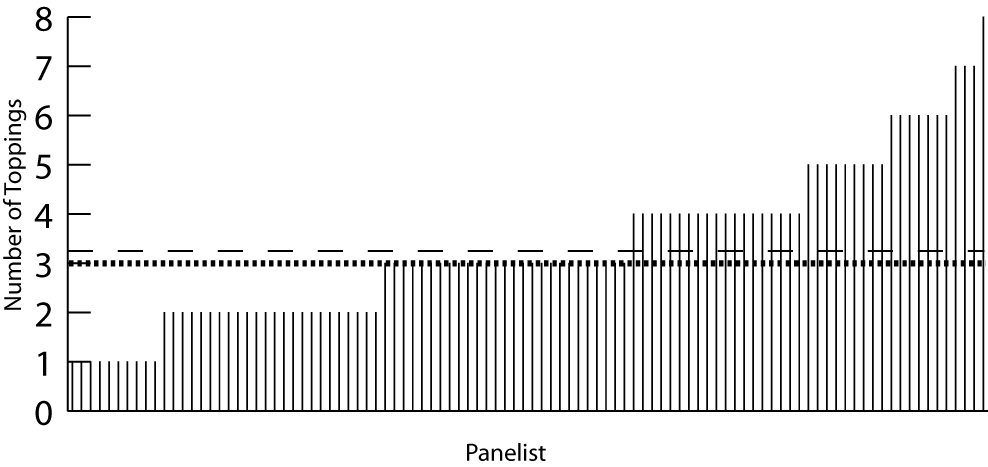
\includegraphics[width=0.9\textwidth]{./img/Figure41.png}
\end{figure}

Part 1 of the survey was completed in 20-35 minutes for each subject.  Figure~\ref{fig:pizzsize} is a histogram showing the number of compatible pairs by percentages of responses.  As mentioned above, we adjusted our threshold to 78 out of 124 panelists, which means that a proportion of people equal to 0.629 had to agree that a pair was compatible for it to be counted as an edge.  An alternative thresholding strategy could decide a threshold based on the proportion itself rather than size of the combination (essentially our method in reverse).  This would allow the investigator to say “we only want pairs accepted by 75\% of the population.”  Dangers of setting the threshold too high or too low are evident in Figure~\ref{fig:pizzsize}.  If the threshold is too strict, Type II error becomes a danger and if it is too lenient Type I error becomes a concern.  As the threshold goes up, you are more likely to miss combinations that may be acceptable.  As the threshold goes down, less compatible cliques are likely to emerge in to the results.  This risk assessment is an important aspect of the experimental design.

\begin{figure}[h!]
\caption[The distribution of responses from Part 1 of the survey.]{The distribution of responses from  Part 1 of the survey.  This shows the number of pairs that people determined were compatible.  The mean proportion was 0.50.}
\label{fig:pizzsize}
\centering
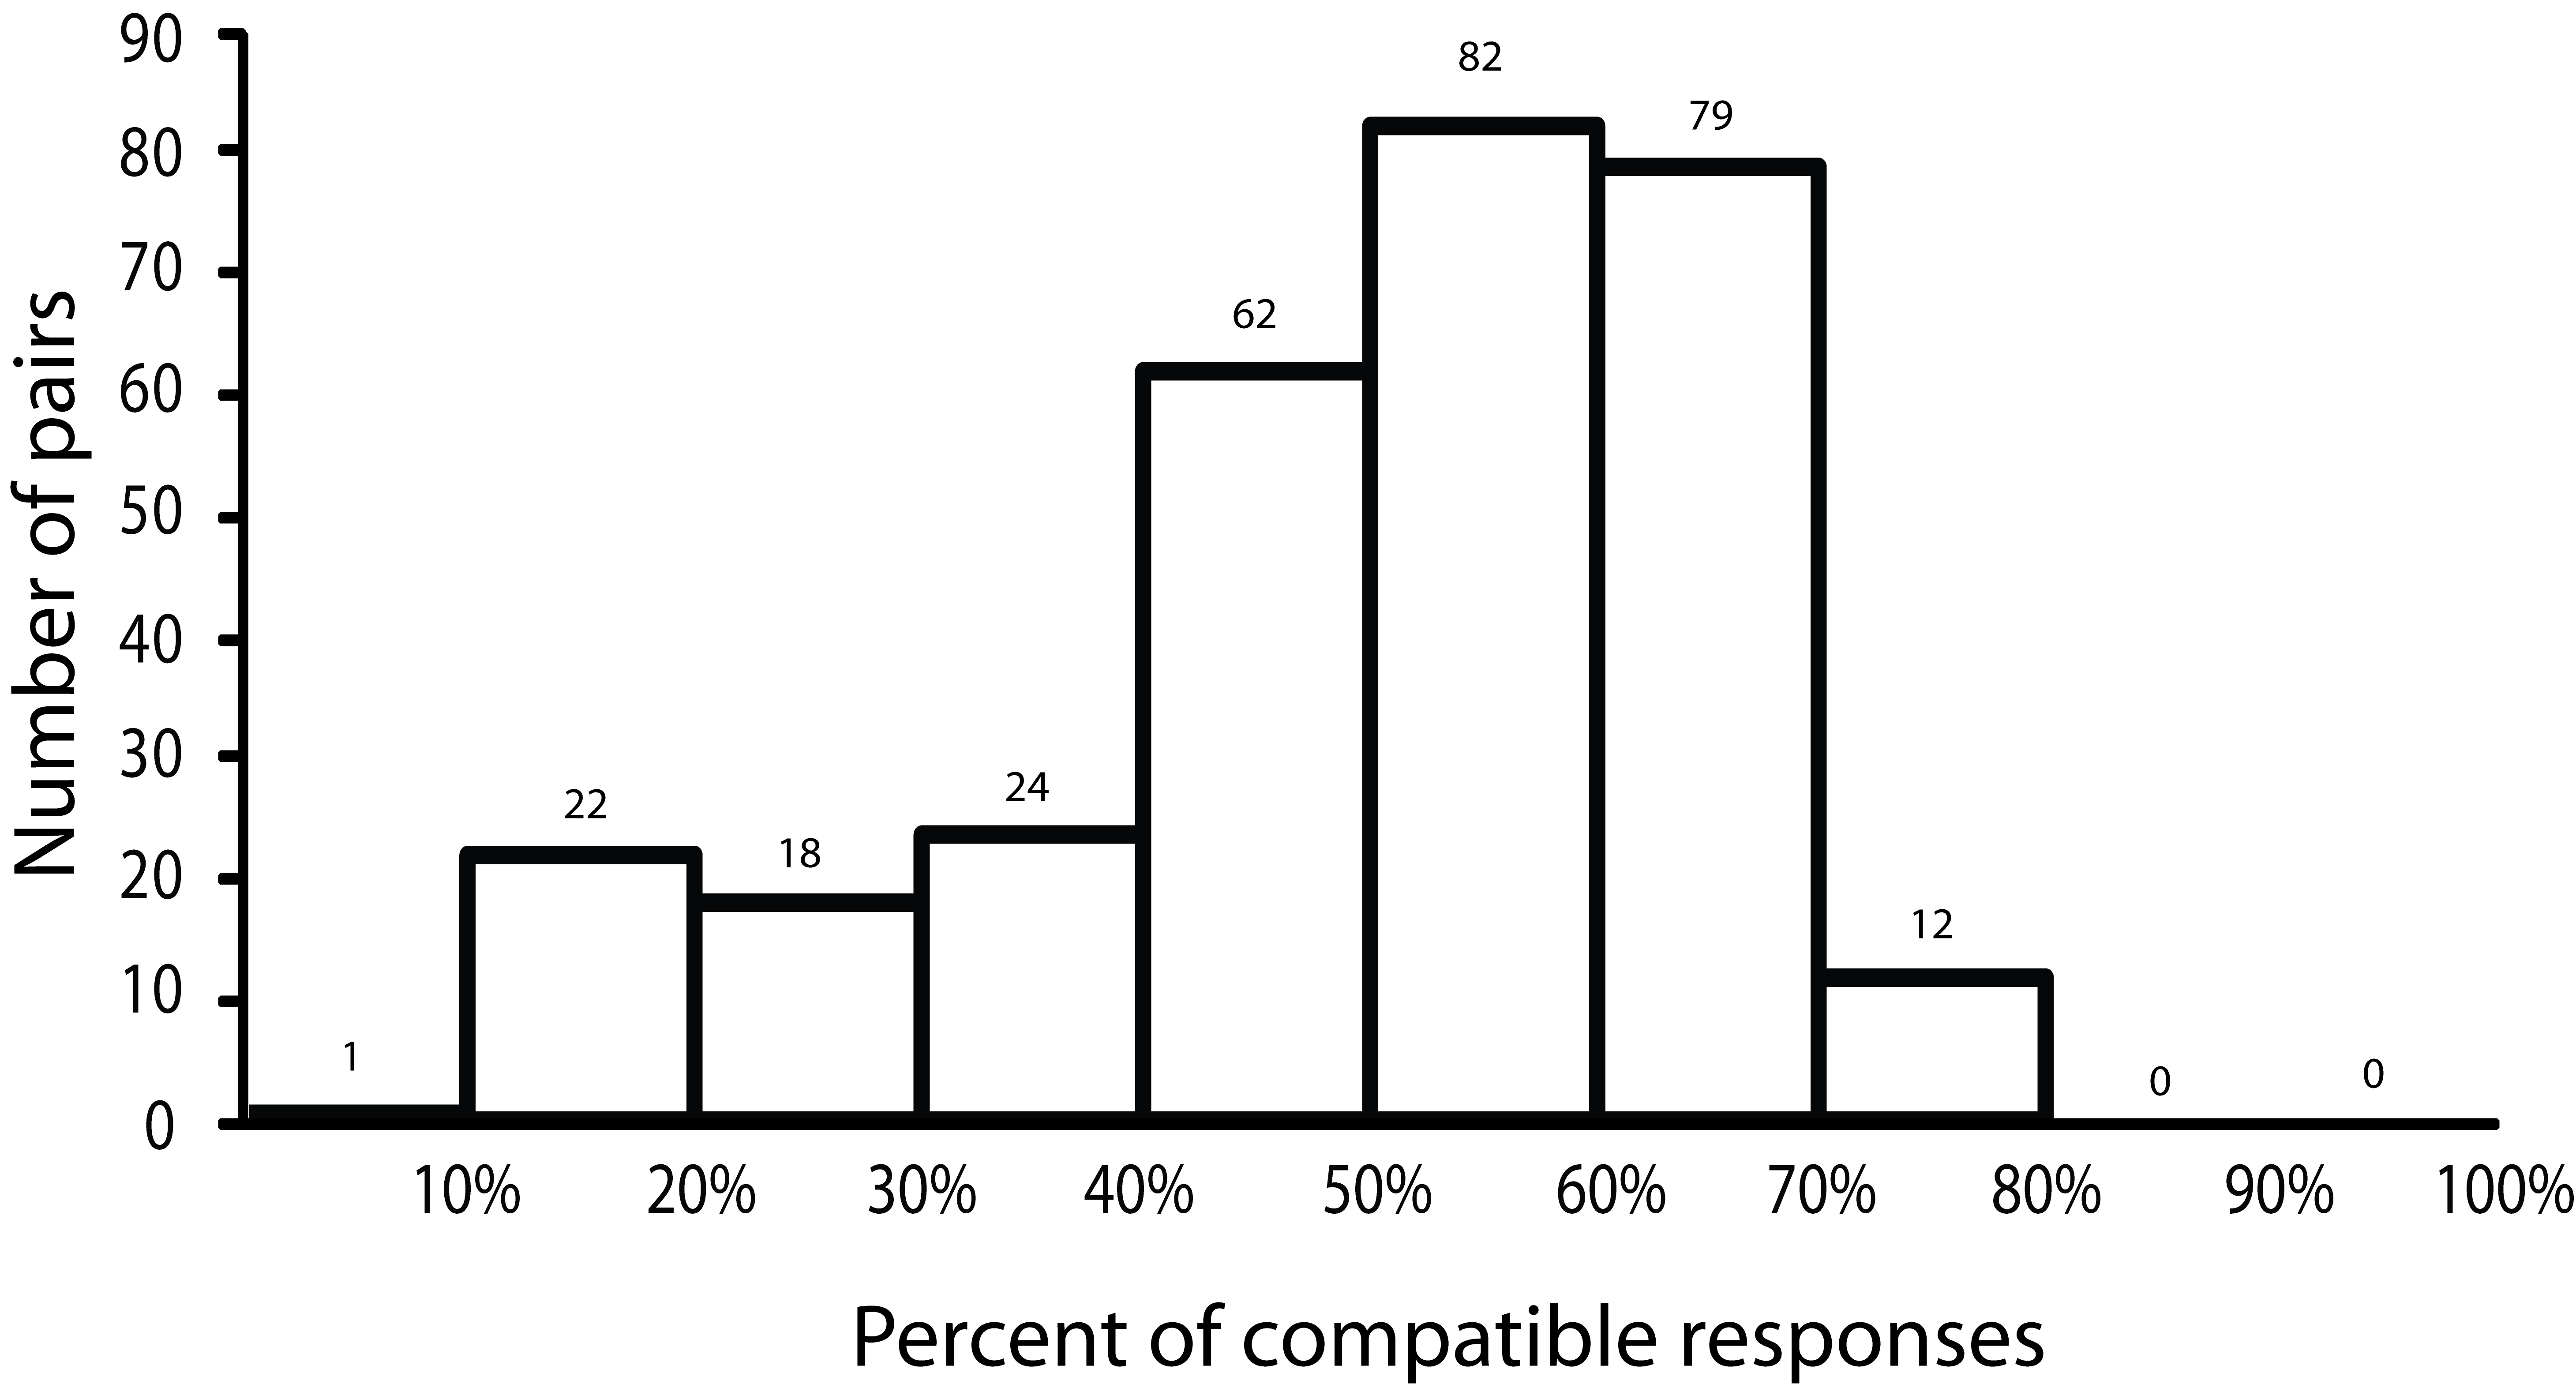
\includegraphics[width=0.9\textwidth]{./img/Figure42.png}
\end{figure}

Once our threshold was applied, 50 out of 300 compatible pairs moved forward in the analysis.  Figure~\ref{fig:pizzedge} shows a graph with edges of the 50 pairs that were used to find larger combinations of compatible pizza toppings. It is evident from this graph that weakly connected toppings like pineapple and red onion are liked in combination with few ingredients, as opposed to ingredients like pepperoni and roasted garlic.  Ingredients such as anchovy and prosciutto that are not connected to other ingredients tend to be liked, but only by themselves (or with ingredients not in our top twenty-five).  From this graph we found the complete set of non-cliques, non-maximal cliques and cliques from sizes one through six.

\begin{table}[h!b!p!]
\caption[Proportion of panelists who chose pizzas of combination sizes 1-6 and overall to be compatible.]{Proportion of panelists who chose pizzas of combination sizes 1-6 and overall to be compatible.  There is a trend to decreasing compatibility as size increases.  }
\label{tab:pizzcompat}
\centering
\begin{tabular}{cccc}
\toprule
{\bf Combination Size} & {\bf Max Cliques} & {\bf Non-max Cliques} & {\bf Non-Cliques}  \\
\midrule
1 & 0.41 & 0.68 & 0.48 \\
2 &  0.64 & 0.69 & 0.42 \\
3 &  0.66 & 0.62 & 0.36 \\
4 &  0.56 & 0.62 & 0.29 \\
5 &  0.57 & 0.58 & 0.26 \\
6 & 0.55 & 0.68 & 0.37 \\
\midrule
Overall & 0.55 & 0.65 & 0.37 \\
\bottomrule
\end{tabular}
\end{table}

The results provide evidence in favor of the SC property.  The overall proportions of YES responses for each of the three groups (non-cliques, non-maximal cliques and maximal cliques) were [0.37, 0.65, 0.55].  These proportions are broken down by combination size in Table~\ref{tab:pizzcompat}.  Maximal cliques of size one (Anchovy, Artichoke, Prosciutto, Jalapeno, Black Olive and Eggplant) were polarizing and had proportions of people who reported purchase interest to a degree more similar to that of the non-cliques than to the cliques. There is also a slight trend across all three groups which indicates that as the number of ingredients increases the probability of a combination being accepted is lower.  This is in line with trend shown in the internet pre-survey in which subjects overwhelmingly listed 1-3 ingredient pizzas as their favorites.

\begin{figure}[h!]
\caption[Edge graph based on thresholded pairwise responses from part 1]{Edge graph based on thresholded pairwise responses from part 1.  Highly connected toppings are highly compatible.}
\label{fig:pizzedge}
\centering
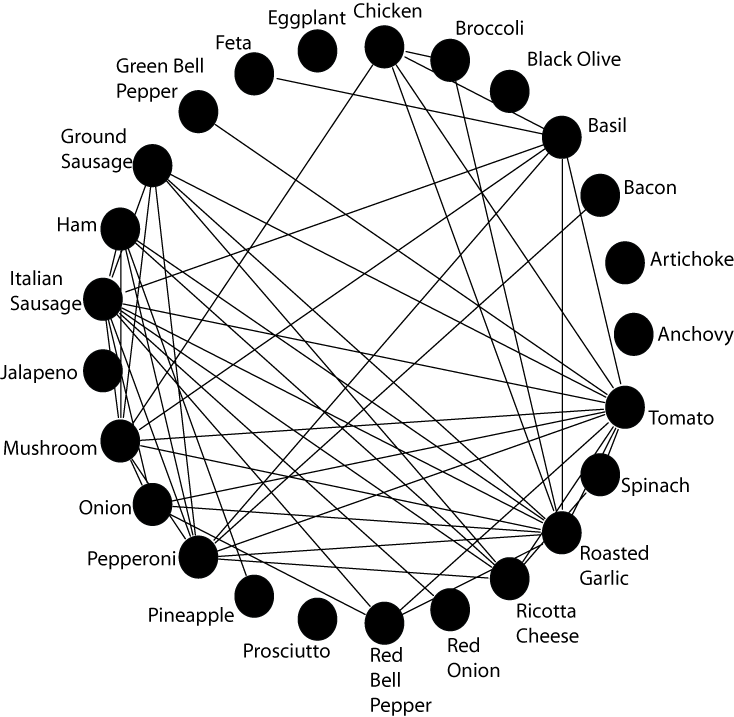
\includegraphics[width=0.9\textwidth]{./img/Figure43.png}
\end{figure}

Figure~\ref{fig:pizzdist} shows the average counts of the number of times a pizza with a given number of toppings was chosen to be compatible for each of the three groups.  As noted above, the max clique of size one is distanced from the rest of the clique responses because these ingredients are polarizing.  The Tukey quick test was designed to assess whether or not two distributions are separated.  There is no significant difference between the maximal-clique and the non-maximal clique groups.  Formal statistical tests cannot be performed to test the difference between the non-cliques and each of the clique groups because the non-parametric tests, including the Wilcox or the Tukey quick test, require that the distributions overlap.  As these distributions do not overlap, we can conclude that the distributions are in fact different and that there is evidence in support of the SC effect.  

\begin{figure}[h!]
\caption[Distribution of average counts of compatible pizzas.]{M:max cliques, C:non-max cliques, N:non-cliques.  Distribution of average counts of compatible pizzas.  Non-cliques were liked less than cliques or max cliques.  There is no difference between the non-max clique and max-clique distributions.}
\label{fig:pizzdist}
\centering
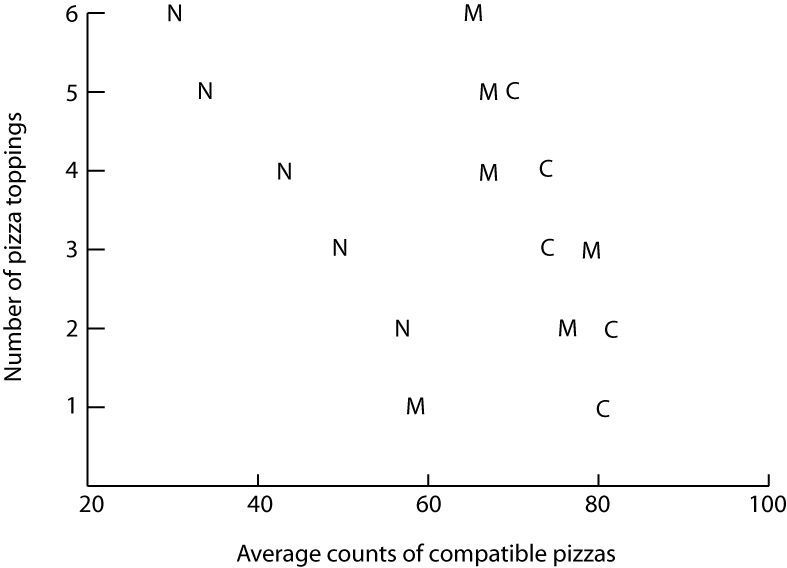
\includegraphics[width=0.9\textwidth]{./img/Figure44.png}
\end{figure}

The combinatorial approach of \citet{Ennis2010} holds promise in allowing food product developers to gain information regarding a large number of food item combinations in a cost efficient manner.  Even so, this technique rests on the crucial SC assumption that needs to be validated before this approach can be confidently employed.  Previously, SC was validated at the individual level \citep{Nestrud2010a}. The research communicated in this present paper demonstrates that SC holds in a group setting and for a different product category.  In this case, the graph theoretic tools allowed us to screen almost a quarter of a million possible combinations down to twenty-one cliques, which were then shown to be of high quality in subsequent testing.  Importantly, these results were obtained in under 30 minutes by asking respondents to generate only three hundred binary responses. 

A future project is to extend the combinatorial approach to meal design, where components from different categories (e.g. starch, protein, vegetable, dessert) are combined to create a highly compatible meal.  This would be useful in the many situations where meals are predetermined, from frozen foods and airline meals to “prix fixe” restaurant value menus and institutional settings such as military and school lunch programs.

\section{Acknowledgements}
The authors thank Effie Nestrud for laboratory assistance and Charles Fayle for invaluable and skillful programming. 

\pagebreak
\renewcommand\bibname{{REFERENCES}} %  will print "REFERENCES" instead of "BIBLIOGRAPHY"
\phantomsection
\addcontentsline{toc}{section}{References} %  adds "REFERENCES" to the table of content
\bibliographystyle{apalike}
\bibliography{library_man}  % uses the references stored in Chapter1Radar.bib
\chapter{A Graph Theoretic Approach to U.S. Army Field Ration Menu Development}
\section{Abstract}
The graph theoretic approach to analyzing food combinations is based on pairwise compatibility information regarding pairs of items.  From this information, which can be collected directly from subjects in a straightforward manner, compatibility information for larger combinations is predicted.  This approach has been validated at the individual and group levels for meals consisting of combinations of items within a single category, but has not yet been applied to meals, such as boxed lunches, that are composed of representatives from distinct categories.  The study presented in this paper extends the graph theoretic approach to such a situation, specifically to military rations known as Meal-Ready-to-Eat or MREs\tm.  MRE\tm menus are composed of 11 different food categories (entr\'{e}e, side, snack, etc.) and there are multiple items available in each category.  From these items, over 22 billion potential menus can be formed.  To identify the most compatible of these menus, pairwise data regarding food item combinations across categories were collected from soldiers familiar with MREs\tm.  These soldiers were asked whether or not pairwise combinations of components were appropriate to combine in a meal.  Using graph theoretic tools, predictions were made of optimal MRE\tm menus and rankings, based on the pairwise information, were created to assist product developers in the improvement of existing menus and the invention of promising new menus.  By applying the graph theoretic approach to meals with multiple categories, and by implementing a ranking approach to assess the compatible menus identified by the graph theoretic technique, this paper adds two unique contributions to the growing body of literature on combinatorial tools in sensory and consumer science.

\section{Introduction}

Consumer driven approaches to menu development have been elusive.  A menu is classically defined as “The portion of food taken at a particular time for the satisfaction of appetite; the quantity usually taken at one time with the purpose of satisfying hunger; a repast” \citep{Webster1913}.  Thus, with regard to a single meal, the menu is the specific set of foods that comprise that meal.  Perhaps unsurprisingly, this definition does not capture the complexity of the meal experience nor give any indication of how to control it.  The food industry has not spent much effort developing meals, rather the focus has been on individual items \citep{Meiselman2000}.  \citet{Meiselman2000} notes that the reason for this gap is because of the complexity of the meal experience which is composed of social, psychological \citep[see esp.][chap. 2]{Lawless2010}  and nutritional factors.  For operational purposes then, we define a meal as a combination of foods from separate categories intended to be consumed together.  
An example menu for a typical southern American meal is smoked pork with barbeque sauce, corn bread, baked beans, coleslaw and lemonade.  The good “categories” in this example are protein, sauce, starch, bread, vegetable and drink respectively.  The reason that these items work well together to create a cohesive “southern American summer barbeque” concept is beyond the scope of this paper, but it includes all of the factors listed above - social: history and tradition, psychological: flavor contrasts \citep{Lawless1977,Lawless1979,Lawless1987,Lawless2010,Lawless2000} and nutritional: protein, fat, starch and a diverse array of nutrients.  The reader could easily come up with a favorite meal from their childhood and also note the complexity as to the reasons “why?” their favorite meal may be considered a good concept.   

When consumer scientists and researchers create meals for commercial production, it is often the complexity of the meal concept that drives development, not considerations of consumer liking.   Many foodservice manufacturers employ research chefs or use internal “experts” to make meal concept decisions.  Other sources for these concepts include teams of food scientists or the established literature.  All of these approaches are notable for the lack of utilizing the intended consumer of the product as a source of information on how the components should be combined together.  

Despite the challenges, there have been some attempts at consumer driven approaches.  Regression based approaches have been used to predict consumer preference for combinations of food items from the preference scores of the individual items \citep{Eindhoven1959,Hedderley1995,Moskowitz1995}.  Unfortunately predictions were poor due to combination effects that this approach neglects to account for, including consumer ethnicity, context, texture, color and frequency of consumption \citep{Eindhoven1959,Marshall2003,Niewind1986,Pilgrim1961}.  

Conjoint analysis is a more advanced regression approach, based on consumer responses, which has achieved some success in predicting consumer preference \citep{Green1978,Luce1964}.  Conjoint analysis predicts combinations by presenting multiple scenarios with different factor levels of the same factor (e.g. different entr\'{e}es or sauces) and finding utility scores for each factor level for its contribution to the overall concept.  Using this approach, an optimal concept or combination of concepts can then be predicted \citep{Moskowitz2006a}.  A more recent advancement in conjoint based approaches allows the consumers themselves to choose the factor levels in which they are interested from a list of alternatives \citep{Liechty2001}.

One notable soldier-based study gives insight into one of the reasons there are challenges with the regression based approaches.  In this study, a bartering metric was used to evaluate how soldiers perceived a meal compared to individual items \citep{Lawless1994}.  Soldiers were observed in the field trading meal items with each other, much as elementary children do during school lunches.  Often, soldiers would build up reserves of a favorite item to use as trading material.  In 1994 this item was the Desert Bar, a chocolate snack product.  Soldiers rated how many Desert bars that they would trade for individual items.  Next, they rated how many desert bars they would trade for an entire meal, composed of the items they had previously rated.  It was observed that the meal was worth less than the sum of the component parts on the “desert bar scale.”  This meal discounting effect has analogies in economics, where, for example, home audio theater systems are cheaper than purchasing separately speakers, a television and a DVD player.  By showing that this effect occurs in foods, Lawless showed that there may be economic-like forces that affect our evaluation of meals.  This discounting effect can be problematic for regression approaches that depend on additivity.  More generally, these challenges together with the complexity of regression based approaches lead us to a relatively new approach to predicting combinations of foods that can be combined to produce desirable meals.

\subsection{Graph Theory}

Graph theory is the mathematical study of connections \citep{Bollobaas1998}.  For our purposes, graph theory  provides a toolkit which, when applied to foods, provides a novel methodology for examining meal component combinations.  In this graph theoretic framework, foods are represented as vertices and foods to which they are connected as edges between them \citep{Ennis2011}.  The advantage of this representation is that it allows us to conduct advanced analyses on how the foods are psychologically connected.  

\citet{Ennisa} have provided a specific graph theoretic methodology for examining consumer responses and creating a cohesive model for predicting how items should be combined together If a consumer scientist is trying to create pizzas for a fixed-item menu at a large restaurant franchising chain, for example, she might have twenty-five toppings to choose from, and she also wants between three to eight toppings on the pizzas.  The exhaustive list of possibilities is 1,807,480 unique pizzas.  The graph theoretic model provides a consumer driven screening approach \citep{Ennis2011} in which this list is screened down to a small number of highly compatible pizzas.  In a typical scenario, this list would then go on to traditional methods of choosing a final list of pizzas to be introduced.  The advantage is that this approach screens out close to two million pizzas, an impossible feat by any other typical product development scenario.  

In the \citet{Ennisa} model, consumers are presented with a list of pairwise combinations of food items and asked whether or not it would be appropriate to combine the two items together.  This unique approach, essentially, fills in the edges of a graph.  Graph theoretic algorithms can then be applied to the responses to predict larger combinations of items.  For example, if a consumer states that the combinations Peach-Vanilla, Vanilla-Orange and Peach-Orange are compatible flavors as pairs, then the larger combination Peach-Vanilla-Orange is a predicted compatible combination.  This larger combination is known as a clique, defined as a completely connected set of vertices \citep{Moon1965}.  However, if one of the pairs, such as Peach-Orange is not compatible, then the larger combination is not compatible.  This concept of seeking fully compatible combinations easily scales up to larger combination sizes depending upon goals.  

This approach was first applied to foods by \citet{Nestrud2010a} in an examination of salad components.  The purpose of the salad study was to highlight and validate the \citet{Ennis2010} approach by presenting consumers with all possible pairs of twenty-five salad ingredients and ask whether or not they thought it would be appropriate to combine the components together on a salad.  Predicted salads of size three to eight were created for each individual based on their responses.  Subjects were then asked whether or not the predicted salads, as well as a selection of random combinations that were predicted to be incompatible (e.g. at least one pair was not connected for the subject), were in fact compatible.  Overwhelmingly, for all combination sizes three through eight, the results supported the compatibility (as measured by appropriateness) of the predicted combinations over the random combinations, thus validating the graph theoretic approach.

\subsection{Meal-Ready-To-Eat or MREs}

The purpose of the MRE\tm, or Meal, Ready to Eat\tm is to provide US military personnel with nutritional sustenance where food service facilities are not available.  Three MREs\tm provide a day’s worth of subsistence.  Each ration is small and portable, occupying no more than 0.08 ft\superscript{3}.   The components of an MRE\tm include an entr\'{e}e, starch, spread, dessert, snacks, bakery item, fruit and a condiment.  Twenty four different MREs\tm are in rotation at any given period and from 1993 through 2010, 216 new items were added to menus and 65 removed \citep{RDECOM2010}.  One of the challenges of development is deciding what existing food items to pair with items that are being considered for introduction.  MRE\tm development is the responsibility of the Combat Feeding Directorate of the U.S. Army Natick R,D and E Center under the authority of the United States Department of Defense.

It has been noted that the “development of new combat rations is fueled by the wants, needs and ideas of Warfighters themselves” \citep{RDECOM2010}.  However, due to complexities of defining meal concepts noted above the primary focus of research has been on the development of individual ration components.  Soldiers provide acceptability information on individual items, and perhaps entire meal concepts, but there has not been a soldier-centric approach to deciding what components best go together to form a meal.  One of the major reasons for this is that there are 22,140,518,400 potential MREs\tm that can be created from the available components!  The current approach is for a small team to decide on which components should be combined, and then these concepts are approved by both soldier surveys and by Department of Defense officials.  Generalizing the graph theoretic approach to our present purposes, however, we propose a new approach for streamlining this type of menu development using input from consumers, who in this case are soldiers.

In this paper then, we present the results of a study designed to extend the graph theoretic screening method of \citet{Ennisa} to more complex food items such as MREs\tm.  In these more complex items, there are inherent restrictions as the combinations being screened are composed of items from many different categories.  In the case of the MRE\tm, for example,  there are eleven different categories and only one item per category is utilized. This restriction has a number of implications for both the experimental design and analysis.  Extending the graph theoretic approach to this restricted environment, we will predict most compatible menus, including two never-before-seen entr\'{e}es.  In addition, we introduce a novel concept of ranking for the candidate menus based on overall compatibility, which enhances previous approaches by not only providing a list of highly compatible menus, but also by providing information that predicts the relative performance of the proposed menus.  

\subsection{Experimental Overview}
The present investigation uses a complex meal item, the MRE\tm, which is composed of eleven categories of food items with many choices of items for each category, and utilizes a graph theoretic optimization strategy to predict most compatible MRE menus..  The concept of appropriateness \citep{Schutz1988} provides us the framework for conducting our study under the correct context.  In particular, we use appropriateness to connect the graph theoretic framework  to the meal experience variables mentioned by \citet{Meiselman2000} (e.g. social and psychological).  To these ends, our primary consumers, military personnel, were recruited on-site in Fort Drum, NY to answer surveys about menu items.  The graph theoretic tools were applied to the responses and ranked MRE\tm menus were presented to the Combat Feeding Directorate for final consideration.

\section{Materials and Methods}
\subsection{Subjects}
Two hundred and seventy active duty personnel (216 male) were recruited at Fort Drum, New York, USA to take part in the survey.  These soldiers comprised a convenience sample of primary consumers.  Their average age was 26 and most of them had been in the armed forces for at least five years.  All had previous experience with MREs\tm and 115 had eaten them at least once in the past six months.  

\subsection{Survey Design}
Eleven different categories of components were considered for evaluation and are listed in Table\ref{tab:mrefood}.

\begin{landscape}
\footnotesize
\begin{longtable}{p{7cm}p{7cm}p{7cm}}
\caption{Categories and MRE\tm items currently available to the Combat Feeding group.} \\
\label{tab:mrefood} \\
\toprule
\endfirsthead
\toprule
\endhead
\midrule
\multicolumn{3}{c}{Continued on next page...} \\
\endfoot
\bottomrule
\endlastfoot
\multicolumn{3}{l}{\bf Entrees} \\
\cmidrule(l){1-1}
Beef Patty, Jalapeno Pepper Jack & Beef Ravioli in Meat Sauce & Beef Roast with Vegetables\\
Beef Stew & Beef Taco Filling & Brisket Entree \\
Cheese Tortellini in Tomato Sauce & Chicken Fajita & Chicken Marsala \\
Chicken, Noodles and Vegetables in Sauce & Chicken Pesto Pasta & Chicken, Pulled with Buffalo Sauce \\
Chicken with Tomatoes and Feta & Chili and Macaroni & Chili and Beans \\
Maple Sausage Wrap & Meatballs in Brown Gravy & Meatballs in Marinara Sauce\\
Mexican Style Chicken Stew & Penne with Veg. Sausage, Spicy Tom. Sce. & Pork Rib, Boneless\\
Pork Sausage Patty, Maple Flavored & Pork Sausage with Gravy & Ratatouille\\
Sloppy Joe Filling & Southwest Style Beef and Black Beans & Spaghetti with Meat and Sauce \\
Spicy Sweet and Sour Pork, Shredded & Szechuan Vegetables and Tofu & Tuna, Lemon Pepper \\
Turkey Chili with Hominy & Vegetable Lasagna & \\
\midrule
\multicolumn{3}{l}{\bf Sides} \\
\cmidrule(l){1-1}
Cornbread Stuffing & Fried Rice & Garlic Mashed Potatoes \\
Granola, with Milk and Blueberries & Macaroni  and Cheese, Mex. Style & Mexican Rice \\
Mexican Corn & Potatoes au Gratin & Potato Cheddar Soup with Bacon \\
Refried Beans & Sante Fe Style Rice and Beans & Vegetable Cous Cous \\
\midrule
\multicolumn{3}{l}{\bf Fruits} \\
\cmidrule(l){1-1}
Apple Pieces in Spiced Sauce & Cherry Blueberry Cobbler & Dried Fruits \\
Fruit, wet pack & &  \\
\midrule
\multicolumn{3}{l}{\bf Desserts} \\
\cmidrule(l){1-1}
Biscuit & Chocolate Banana Muffin Top & Cookies\\
Corn Bread & Filled Bakery Pastry & First Strike Bar\\
Fudge Brownie with Chocolate Drops & Maple Muffin Top & Pancake\\
Pound Cake & Pudding, Instant & Ranger Bar\\
Strawberry Dessert Bar & Sugar Cookie, Patriotic & Toaster Pastry\\
\midrule
\multicolumn{3}{l}{\bf Snacks} \\
\cmidrule(l){1-1}
Baked Snack Cracker, Cheddar & Beef Snacks & Cheese Filled Crackers\\
Cheese Filled Pretzels & Corn Nuts & Nuts\\
Pretzel Sticks & Raisin Nut Mix & Raisin Nut Mix with Chocolate Disks\\
Turkey Pepperoni & Turkey Snacks &\\
\\
\multicolumn{3}{l}{\bf Bakery Items} \\
\cmidrule(l){1-1}
Chipotle Snack Bread & Crackers, Plain & Crackers, Vegetable\\
Multigrain Snack Bread & Tortillas & Wheat Snack Bread\\
White Wheat Snack Bread & & \\
\midrule
\multicolumn{3}{l}{\bf Spreads} \\
\cmidrule(l){1-1}
Apple Butter & Cheese Spread, Pizza & Cheese Spread, Plain\\
Cheese Spread, Taco & Cheese Spread, Bacon & Cheese Spread, Jalapeno Pepper\\
Jelly or Jam & Peanut Butter, Chocolate & Peanut Butter, Chunky\\
Peanut Butter, Smooth & & \\
\midrule
\multicolumn{3}{l}{\bf Condiments} \\
\cmidrule(l){1-1}
Barbecue Sauce & Barbecue Seasoning & Butter Granules\\
Hot Sauce & Ketchup & Mayonnaise, Fat Free\\
Mustard, Yellow & Picante Sauce & Pizza Seasoning\\
Red Pepper, Ground & Seasoning Blend, Salt Free, Herbs and Citrus & Steak Sauce\\
Table Syrup & & \\
\\
\\
\\
\multicolumn{3}{l}{\bf Candy} \\
\cmidrule(l){1-1}
Caffeinated Mints & Chocolate Toffee Rolls & Plain Chocolate Disks, Chocolate with Peanut Ovals and Peanut Butter Disks\\
Tropical and Berry Fruit Disks, Cherry Licorice\\
\midrule
\multicolumn{3}{l}{\bf Beverages (main)} \\
\cmidrule(l){1-1}
Beverage Base, sugar free & Beverage Base, Carbohydrate and Vitamin C & Beverage Powder, carbohydrate and electrolyte\\
Cocoa Beverage Powder & Cocoa Beverage Powder, Chocolate Hazelnut & Coffee, Flavored\\
Dairy Shake & Lemon Tea &\\
\midrule
\multicolumn{3}{l}{\bf Beverages (accessory)} \\
\cmidrule(l){1-1}
Apple Cider & Coffee & Milk, Non-Fat\\

\end{longtable}
\end{landscape}

The number of items within each category varied from a high of thirty-two (for entr\'{e}es) to a low of four (for fruits).  In a previous graph theoretic investigation \citep{Nestrud2010a}, all subjects were able to evaluate all possible salad ingredient pairs.  This was not possible in the current investigation due to time constraints and the fact that in our present case there were over 10,000 pairs that could be formed across categories.  Using the expertise of the Combat Feeding Directorate, we reduced the list of all possible pairs down to a reasonable number for evaluation.  The a priori conclusion was made to not consider candy or either beverage categories in combination with anything else, because the experts in Combat Feeding felt that it was reasonable to assume these categories were rarely, if ever, taken into account by the soldiers when determining overall compatibility.  Further reductions were made by selectively choosing which pairs of categories were unimportant to overall compatibility and eliminating those.  Eight of the twenty-six possible category pairs were concluded to be the most important.  The final category pairs were: Bakery-Spread, Entr\'{e}e-Bakery, Entr\'{e}e-Condiment, Entr\'{e}e-Spread, Entr\'{e}e-Starch, Fruit-Dessert, Fruit-Snack and Starch-Fruit, containing a total of 104 individual items.

An exhaustive list was made of all 1370 between-category pairs.  This was the final list of pairs to be evaluated by the soldiers.  The complete set of pairs was randomized both with respect to order within pairs and between pairs and the resultant list was split into four surveys (in other words, four soldiers completing the survey corresponded to the entire set of pairs being evaluated once).  This partitioning of the pairs allowed each respondent to evaluate 342 or 343 pairs, a reasonable number.  Demographic information was also included on each survey.  A truncated example survey is presented in Figure~\ref{fig:mresurvey}.  The instructions on the first page set the conditions for the evaluation:

\noindent
{\it The purpose of this survey is to help us with designing better MREs. In this survey you will encounter pairs of items that may be packaged together in an MRE.

\noindent
For each row on the following pages, please fill in YES if you would want to consume ITEM A at the same meal as ITEM B.

\noindent
Please fill in NO if you would NOT want to consume ITEM A at the same meal as ITEM B.}

\begin{figure}[h!]
\caption{Example MRE survey.}
\label{fig:mresurvey}
\centering
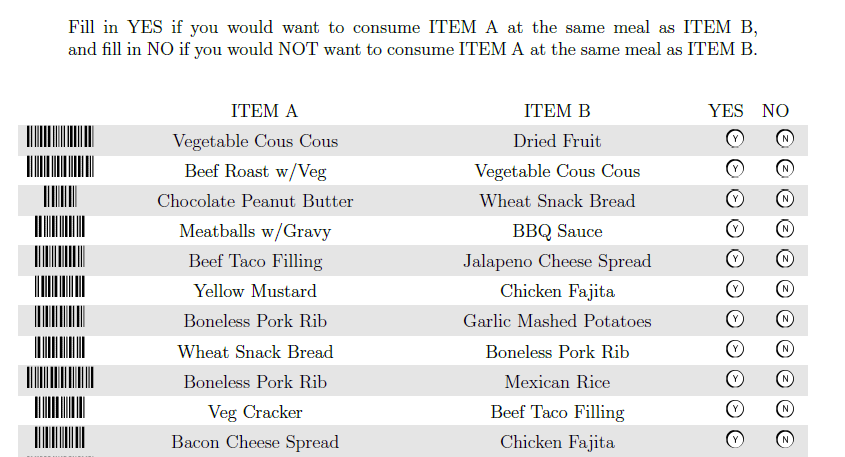
\includegraphics[width=0.9\textwidth]{./img/Figure51.png}
\end{figure}

\subsection{Data Analysis}
Due to some incomplete surveys, all pairs were evaluated between 61 and 69 times each.  Total proportions reflecting how frequently each pair was chosen as compatible were computed.  These proportions were used to create thirty-two individual lower triangular matrices, one per entr\'{e}e, as the entr\'{e}e is the centerpiece of the MRE\tm menu.  The rows and columns of these matrices corresponded to the food items in the study, with the (i,j) entry containing the compatibility proportion for the i\superscript{th} food item with the j\superscript{th} food item, according to a predetermined ordering of the items.  Where cross-category pairs were eliminated as a survey design consideration, proportions equal to 1 were input into the matrices.  All within-category pairs (e.g. Snack-Snack) were filled in with zeroes to denote these within-category pairs as incompatible and meals with multiple items from the same category impossible.

For each entr\'{e}e, we followed the following algorithm for determining the compatible meals associated with the entr\'{e}e.  The purpose of this algorithm is to determine which cutoff for compatibility we should use to define a pair of food items as “connected” from a graph theoretic standpoint.  First, we followed the following process for each of the proportion values in the matrix for the entr\'{e}e under consideration, beginning with the largest proportion and proceeding in decreasing order.  For each proportion, any smaller proportions were temporarily set to 0, meaning that the corresponding pair of food items was to be considered, for the moment, as disconnected.  Similarly, any equal or larger proportions were temporarily set to 1, meaning that the corresponding pair of food items was to be considered, for the moment, as connected.  In this temporary state, we found the cliques associated with this iteration, reset our values, and started over at the next proportion.  Recall that a clique is a fully connected combination, so in this case a clique of food items corresponds to a fully compatible meal.  As we stepped down through the proportions, we stopped our search as soon as cliques of size eight, the size of the MRE\tm menu, were found.  This approach ensured that we found the MRE\tm menus of maximum compatibility, as further relaxing our cutoff for connectedness would have yielded more, less compatible, menus.  

To evaluate the quality of these menus, we used a novel ranking approach.  Having found the fully compatible menus in our previous step, we then calculated the average proportion of compatibility for each compatible menu.  More specifically, for all inter-category pairs there was a proportion of compatibility based on the original soldier responses.  For each proposed menu, we averaged those proportions, ignoring zeroes and ones, thus providing a valuable metric for determining the best menus per entr\'{e}e.  All data analysis was conducted with R 2.10.0 and surveys were created using custom LaTeX templates and the R Sweave package.  Barcodes were used to efficiently scan in responses.

\section{Results and Discussion}
The top MRE\tm menus for each of the 32 entr\'{e}es are listed in Table~\ref{tab:mremeals}.  The score for each menu is the average proportion of compatibility between each pair that was evaluated by the soldiers for that menu.  The menu with the highest compatibility score contains Chili with Beans, with a score of 0.8160.  The  Chili with Beans menu currently in production is paired with Mexican Corn as a side, Cheese Spread and ground red pepper as a seasoning.  By replacing these items with those predicted from Table~\ref{tab:mremeals}, we expect the overall compatibility of the menu to increase along with, we predict, the overall liking of the menu.  The lowest scored menu contains Szechuan Vegetables with Tofu (score=0.6377).  This means that there was no good combination of items, from all of the possible items presented, that would create a highly compatible MRE\tm meal using this entr\'{e}e.  Rather than develop new MRE\tm menu items across the board to increase compatibility, the recommendation would be to eliminate this menu item and to focus efforts on the entr\'{e}es with medium range compatibility scores to increase compatibility and acceptance.

\begin{landscape}
\footnotesize
\begin{longtable}{p{3.0cm}p{3.7cm}p{2.2cm}p{2.0cm}p{2.3cm}p{0.8cm}p{1.5cm}p{2.2cm}p{0.8cm}}
\caption{List of No. 1 meals for each of the 32 entr\'{e}e items.  } \\
\label{tab:mremeals} \\
\endfirsthead
\midrule
{\bf Entree} & {\bf Side} & {\bf Seasoning} & {\bf Bakery} & {\bf Spreads} & {\bf Fruits} & {\bf Desserts} & {\bf Snacks} & {\bf Score}\\
\midrule
\endhead
 \multicolumn{3}{c}{Continued on next page...} \\
\endfoot
\bottomrule
\endlastfoot
\toprule
{\bf Entree} & {\bf Side} & {\bf Seasoning} & {\bf Bakery} & {\bf Spreads} & {\bf Fruits} & {\bf Desserts} & {\bf Snacks} & {\bf Score}\\
\midrule
Chili with Beans & Mex. Mac and Cheese & Herb-Citrus Seasoning & Crackers, Plain & Peanut Butter, Chunky & Fruit (Wet) & Cookies & Cheese-Filled Pretzels & 0.8160 \\
\midrule
Pork Ribs & Garlic Mashed Potatoes & Herb-Citrus Seasoning & Crackers, Plain & Peanut Butter, Chunky & Fruit (Wet) & Cookies & Cheese-Filled Pretzels & 0.8151 \\
\midrule
Beef Roast, Veg. & Cornbread Stuffing & Red Pepper & Crackers, Plain &  Peanut Butter, Chunky & Fruit (Wet) & Cookies & Cheese-Filled Pretzels & 0.8069 \\
\midrule
Buffalo Chicken & Garlic Mashed Potatoes & Red Pepper & Crackers, Plain &  Peanut Butter, Chunky & Fruit (Wet) & Cookies & Cheese-Filled Pretzels & 0.8027 \\
\midrule
Beef Taco Filling & Mexican Rice & Red Pepper & White Bread & Peanut Butter, Chocolate & Fruit (Wet) & Cookies & Cheese-Filled Pretzels & 0.8011 \\
\midrule
Chili \& Macaroni & Potato, Cheddar \& Bacon Soup & Herb-Citrus Seasoning & Crackers, Plain & Peanut Butter, Chunky & Fruit (Wet) & Cookies & Cheese-Filled Pretzels & 0.8005 \\
\midrule
Chicken Marsala & Garlic Mashed Potatoes & Hot Sauce & Crackers, Plain & Peanut Butter, Chunky & Fruit (Wet) & Cookies & Cheese-Filled Pretzels & 0.7989 \\
\midrule
Meatballs,Marinara Sauce & Potatoes au Gratin & Hot Sauce & Crackers, Plain & Peanut Butter, Chunky & Fruit (Wet) & Cookies & Cheese-Filled Pretzels & 0.7919 \\
\midrule
Beef Brisket, Gravy & Garlic Mashed Potatoes & BBQ Seasoning & Crackers, Plain & Peanut Butter, Chunky & Fruit (Wet) & Cookies & Cheese-Filled Pretzels & 0.7915 \\
\midrule
Spaghetti, Meat \& Sauce & Garlic Mashed Potatoes & Red Pepper & Crackers, Plain & Peanut Butter, Chunky & Fruit (Wet) & Cookies & Cheese-Filled Pretzels & 0.7891 \\
\midrule
Spicy Sweet \& Sour Pork & Fried Rice & Herb-Citrus Seasoning & Crackers, Plain & Peanut Butter, Chunky & Fruit (Wet) & Cookies & Cheese-Filled Pretzels & 0.7891\\
\midrule
Beef Stew & Garlic Mashed Potatoes & Red Pepper & Crackers, Plain & Peanut Butter, Smooth & Fruit (Wet) & Filled Bakery & Cheese-Filled Pretzels & 0.7869 \\
\midrule
Chicken, Tomatoes \& Feta & Fried Rice & Herb-Citrus Seasoning & Crackers, Plain & Peanut Butter, Chunky & Fruit (Wet) & Cookies & Cheese-Filled Pretzels & 0.7847 \\
\midrule
Chicken, Noodles \& Vegetables & Garlic Mashed Potatoes & Hot Sauce & Crackers, Plain & Peanut Butter, Chunky & Fruit (Wet) & Cookies & Cheese-Filled Pretzels & 0.7819 \\
\midrule
Sloppy Joe & Garlic Mashed Potatoes & Herb-Citrus Seasoning & Wheat Bread & Peanut Butter, Smooth & Fruit (Wet) & Cookies & Cheese-Filled Pretzels & 0.7810 \\
\midrule
Chicken Fajita & Mexican Rice & Herb-Citrus Seasoning & White Bread & Peanut Butter, Chocolate & Fruit (Wet) & Cookies & Cheese-Filled Pretzels & 0.7769 \\
\midrule
Meatballs in Brown Gravy & Garlic Mashed Potatoes & Herb-Citrus Seasoning & Crackers, Plain & Peanut Butter, Chunky & Fruit (Wet) & Cookies & Cheese-Filled Pretzels & 0.7753 \\
\midrule
Beef Ravioli in Meat Sauce & Garlic Mashed Potatoes & Herb-Citrus Seasoning & Crackers, Plain & Peanut Butter, Chunky & Fruit (Wet) & Cookies & Cheese-Filled Pretzels & 0.7722 \\
\midrule
Beef Patty, Pepper Jack & Potatoes au Gratin & BBQ Sauce & Wheat Bread & Peanut Butter, Smooth & Fruit (Wet) & Cookies & Cheese-Filled Pretzels & 0.7719 \\
\midrule
Cheese Tortellini in Tomato Sauce & Potato, Cheddar \& Bacon Soup & Red Pepper & Crackers, Plain & Peanut Butter, Chunky & Fruit (Wet) & Cookies & Cheese-Filled Pretzels & 0.7657 \\
\midrule
Turkey Chili with Hominy & Garlic Mashed Potatoes & Hot Sauce & Crackers, Plain & Peanut Butter, Chunky & Fruit (Wet) & Cookies & Cheese-Filled Pretzels & 0.7596 \\
\midrule
Tuna with Lemon Pepper & Garlic Mashed Potatoes & Herb-Citrus Seasoning & Crackers, Plain & Peanut Butter, Chunky & Fruit (Wet) & Cookies & Cheese-Filled Pretzels & 0.7574 \\
\midrule
Mex. Chicken Stew & Mex. Mac and Cheese & Hot Sauce & Crackers, Plain & Peanut Butter, Chunky & Fruit (Wet) & Cookies & Cheese-Filled Pretzels & 0.7570 \\
\midrule
Pork Sausage with Gravy & Garlic Mashed Potatoes & Herb-Citrus Seasoning & Crackers, Plain & Peanut Butter, Chunky & Fruit (Wet) & Cookies & Cheese-Filled Pretzels & 0.7531 \\
\midrule
Southwest Beef \& Black Beans & Fried Rice & Hot Sauce & Crackers, Plain & Peanut Butter, Chunky & Fruit (Wet) & Cookies & Cheese-Filled Pretzels & 0.7422 \\
\midrule
Chicken Pesto Pasta & Garlic Mashed Potatoes & Herb Citrus Seasoning & Multigrain Bread & Peanut Butter, Chunky & Fruit (Wet) & Cookies & Cheese-Filled Pretzels & 0.7416 \\
\midrule
Vegetable Lasagna & Potatoes au Gratin & Hot Sauce & Crackers, Plain & Peanut Butter, Chunky & Fruit (Wet) & Cookies & Cheese-Filled Pretzels & 0.7391 \\
\midrule
Penne with Sausage, Spicy Tomato Sauce & Garlic Mashed Potatoes & Red Pepper, Ground & Vegetable Crackers & Peanut Butter, Chunky & Fruit (Wet) & Cookies & Cheese-Filled Pretzels & 0.7360 \\
\midrule
Ratatouille & Garlic Mashed Potatoes & Red Pepper & Crackers, Plain & Peanut Butter, Chunky & Fruit (Wet) & Cookies & Cheese-Filled Pretzels & 0.7301 \\
\midrule
Pork Sausage Patty, Maple Flavored & Granola & Table Syrup & Wheat Bread & Peanut Butter, Smooth & Fruit (Wet) & Cookies & Cheese-Filled Pretzels & 0.7281 \\
\midrule
Maple Sausage Wrap & Granola & Table Syrup & Multigrain Bread & Peanut Butter, Chunky & Fruit (Wet) & Cookies & Cheese-Filled Pretzels & 0.7100 \\
\midrule
Szechuan Vegetables \& Tofu & Fried Rice & Herb Citrus Seasoning & Vegetable Crackers & Peanut Butter, Chunky & Fruit (Wet) & Cookies & Cheese-Filled Pretzels & 0.7377 \\
\end{longtable}
\end{landscape}

There were two entr\'{e}e items that were being considered for introduction.  Field tests to evaluate the palatability of the new entr\'{e}es typically are challenging, because the development group, by necessity, would make educated guesses as to which of the other meal items they should pair with the entr\'{e}e to create the MRE\tm meal.  We know that flavor contrast effects and other contextual effects are important to our overall concept of the meal, so it is important to choose the entire meal carefully.  Our study incorporated the two new entr\'{e}es, which were the Beef Patty and the Beef Taco Filling.  The best predicted menus are shown in Table~\ref{tab:mremeals}.  Both menus have strong meal proportion scores, and the Beef Taco Filling is one of only six entr\'{e}es with a score above 0.80.  This gives evidence that this particular meal combination is likely to be highly successful.  

Table~\ref{tab:mrechili} contains the top 10 MRE\tm menus for the Chili Mac entr\'{e}e.  This table illustrates the value of this approach as a screening tool and not as an ultimate solution providing a single answer.  For example, in Table~\ref{tab:mremeals} we notice that there is very little variation in some of the categories, such as Desserts and Spreads.  However, using Table~\ref{tab:mrechili} we can see that we could use the 8th ranked combination rather than the 1st ranked item, introduce some variety into this category, and the compatibility score drops only 0.50\%.  

\begin{landscape}
\footnotesize
\begin{longtable}{p{0.5cm}p{4cm}p{4cm}p{2cm}p{2.3cm}p{0.8cm}p{1.5cm}p{2.2cm}p{0.8cm}}
\caption{Top 10 menus for the Chili-mac entree item } \\
\label{tab:mrechili}
\endfirsthead
\midrule
{\bf Rank} & {\bf Side} & {\bf Seasoning} & {\bf Bakery} & {\bf Spreads} & {\bf Fruits} & {\bf Desserts} & {\bf Snacks} & {\bf Score}\\
\hline
\endhead
\multicolumn{3}{c}{Continued on next page...} \\
\endfoot
\bottomrule
\endlastfoot
\toprule
{\bf Rank} & {\bf Side} & {\bf Seasoning} & {\bf Bakery} & {\bf Spreads} & {\bf Fruits} & {\bf Desserts} & {\bf Snacks} & {\bf Score}\\
\midrule
1 & Potato, Cheddar \& Bacon Soup & Herb-Citrus Seasoning & Crackers, Plain & Peanut Butter, Chunky & Fruit (Wet) & Cookies & Cheese-filled Pretzels & 0.8005\\
\midrule
2 & Potato, Cheddar \& Bacon Soup & Herb-Citrus Seasoning & Wheat Bread & Peanut Butter, Chocolate & Fruit (Wet) & Cookies & Cheese-filled Pretzels & 0.7988\\
\midrule
3 & Potato, Cheddar \& Bacon Soup & Red Pepper & Crackers, Plain & Peanut Butter, Chunky & Fruit (Wet) & Cookies & Cheese-filled Pretzels & 0.7975\\
\midrule
4 & Potato, Cheddar \& Bacon Soup & Herb-Citrus Seasoning & Crackers, Plain & Cheese Spread, Plain & Fruit (Wet) & Cookies & Cheese-filled Pretzels & 0.7973\\
\midrule
5 & Potato, Cheddar \& Bacon Soup & Herb-Citrus Seasoning & Crackers, Plain & Peanut Butter, Chunky & Fruit (Wet) & Filled Bakery & Cheese-filled Pretzels & 0.7968\\
\midrule
\\
\\
\\
\\

6 & Potato, Cheddar \& Bacon Soup & Herb-Citrus Seasoning & Wheat Bread & Jelly or Jam & Fruit (Wet) & Cookies & Cheese-filled Pretzels & 0.7968\\
\midrule
7 & Potato, Cheddar \& Bacon Soup & Red Pepper & Wheat Bread & Peanut Butter, Chocolate & Fruit (Wet) & Cookies & Cheese-filled Pretzels & 0.7955\\
\midrule
8 & Potato, Cheddar \& Bacon Soup & Herb-Citrus Seasoning & Wheat Bread & Peanut Butter, Chocolate & Fruit (Wet) & Filled Bakery & Cheese-filled Pretzels & 0.7943\\
\midrule
9 & Potato, Cheddar \& Bacon Soup & Red Pepper & Crackers, Plain & Cheese Spread, Plain & Fruit (Wet) & Cookies & Cheese-filled Pretzels & 0.7943\\
\midrule
10 & Potato, Cheddar \& Bacon Soup & Herb-Citrus Seasoning & Crackers, Plain & Cheese Spread, Plain & Fruit (Wet) & Filled Bakery & Cheese-filled Pretzels & 0.7942\\
\end{longtable}
\end{landscape}

In a similar vein and perhaps unsurprisingly since the respondents were a typical cross-section of soldiers, some of the entr\'{e}es that are designated vegetarian have been combined with meat based side items (e.g. Penne with Vegetables and Potato, Cheddar and Bacon soup).  This is another example where the expertise of the meal developers is critical to find and further screen out these incompatible combinations.  Alternatively, this expertise could be used to further restrict the pairs included in the test design, in this case not presenting soldiers with any pairs involving vegetarian and non-vegetarian items simultaneously.  Other restrictions specific to MREs\tm that are not incorporated into the model and are left for screening include size of components, nutritional restrictions, variety  and intended use.  It is worth noting that tools from discrete mathematics, specifically algorithms that approach the so-called “knapsack” problem could be used to address these problems \citep{Martello1990}.  As currently executed, however, the current proposed meal development approach provides an excellent tool for evaluating and screening billions of potential meals.

One possibility worthy of investigation is that compatibility scores  might be correlated with whether or not a menu item is liked at all.  That is, if an item is compatible with large numbers of other items, it may well be a highly liked item.  Alternatively, an item with low compatibility with other items, e.g. the Szechuan Vegetables with Tofu item, in the present study might well be simply a disliked item and no combination at all would make the score of this entr\'{e}e high.  A useful follow-up study could investigate these correlations.  If there is liking information embedded in the compatibility information, this approach would prove even more powerful.

With the addition of categories to the \citet{Ennisa} model, we have provided a way to measure complex information about meal experience.  This methodology takes a meta-level approach to meal design by looking at which items are combined together most often using the consumers, in this case soldiers, themselves to define the criteria for connectivity.  As long as consumers have some sort of common understanding of what should be combined together, no matter the reason, this methodology will capture compatibility patterns and provide concrete recommendations for highly compatible menus.  Even though this approach does not specifically concern itself with the social, psychological and nutritional factors that \citet{Meiselman2000} proposes as building blocks of the meal experience, by incorporating the graph theoretic approach with an appropriateness framework and internal expertise, all three of Meiselman’s factors are accounted for.  	

\section{Acknowledgements}
We thank Daniel Ennis and Charles Fayle for their support, ideas and expertise in the execution of this investigation.

\pagebreak
\renewcommand\bibname{{REFERENCES}} %  will print "REFERENCES" instead of "BIBLIOGRAPHY"
\phantomsection
\addcontentsline{toc}{section}{References} %  adds "REFERENCES" to the table of content
\bibliographystyle{apalike}
\bibliography{library_man}  % uses the references stored in Chapter1Radar.bib

\chapter{General Discussion and Conclusions}
\section{Discussion}
This research program provides the consumer science community with the first empirical investigation using graph theory to represent food connections.  It is believed that this methodology will be further developed and become a standard portion of the sensory scientists’ toolbox. 
The questioning procedure has subjects rate pairwise compatibility information on popular ingredients.  In the graph theoretic model this builds up the connectivity information necessary to build a graph (see Figures~\ref{fig:saladgraph} and~\ref{fig:pizzedge}).  Graphs are dynamic mathematical representations that have numerous analyses available for them.  The implementation of clique finding algorithms to explore larger combinations is only the tip of the iceburg of what can be done.  

The open challenge of finding optimal combinations of food components for various applications (MREs\tm, frozen meals, pizzas, salads, flavor combinations for yogurts/smoothies, etc.) led to the natural application of cliques to predict those combinations.  The usefulness of this approach was dependent on validation, however.  First, the salad study showed, for individuals, that pairwise information does provide good predictions of overall.  Table~\ref{tab:propsalad} illustrates that the majority of people chose predicted combinations over random combinations.  In fact, out of the 63 people in the study only 3 chose more non-cliques than cliques as being compatible.  This shows the potential of the method's remarkable abilities to create predictions.  

Even though the methodology was shown to hold at the individual level, it was important to provide methodology to combine individual group data together to form a group consensus (See Table~\ref{tab:pizztri}) and also show that, when these data were combined, that too much information was not lost.  Table~\ref{tab:pizzcompat} shows that in fact the scaling up does hold at the group level as well.  It is important to note, however, that these concepts were only validated for a pizza and salads and that, while probable, it is not a given that these results would be mirrored for all possible categories of foods.  Thus, Chapter IV also serves as a template for validating the method for other product categories.  Once validated, the method can be used faithfully to measure changes in perception over time, predict new combinations of foods, investigate competitors products and optimize product lines.

Chapter V introduced an extension to the experiment which served multiple purposes in this research program.  First and foremost we introduced methodology to extend the graph theoretic approach to menus – that is, optimizing items from different categories.  Second, by using MREs\tm, we chose an incredibly complex product with 11 different categories of food items and over 100 different components.  This stress-tested the method, as typical meals in other applications (schools, prisons, frozen meals, etc.) have 3 or 4 categories and only a handful of options in each category.  We also chose to focus on the entrée as the centerpiece of these meals and build our menus around the entrée frame-of-reference (Table~ref{tab:mremeals}).  This approach, combined with the ability to rank menus, provides extremely useful information to the product developer to help screen potential new menus. 

There are a number of obvious follow-up studies that should take place.  First, it is desired to take our predicted MRE\tm menus back to soldiers and run a validation experiment to test if our predictions fare better than random combinations.  We would also like to correlate this with individual liking information for the various components, as this would allow us to discover if there is a combination effect or not.  Second, these results should be replicated with additional product systems and with different groups of people.  Do children form the same complex pairwise relationships with foods?  Or are more simplistic regression based approaches good enough?  

\section{Conclusions}
These investigations have shown the potential for the graph theoretic approach to revolutionize the way combinations of foods are mathematically represented (from the analysts point of view) and developed (from the food product developer/ food scientist’s point of view).  The first two investigations have validated the necessary underlying assumptions needed for the method to be trusted.  The final investigation shows a complex real world application and demonstrates the type of results that can be expected when employing this methodology. 



\end{document}
